% Options for packages loaded elsewhere
\PassOptionsToPackage{unicode}{hyperref}
\PassOptionsToPackage{hyphens}{url}
%
\documentclass[
]{article}
\usepackage{amsmath,amssymb}
\usepackage{iftex}
\ifPDFTeX
  \usepackage[T1]{fontenc}
  \usepackage[utf8]{inputenc}
  \usepackage{textcomp} % provide euro and other symbols
\else % if luatex or xetex
  \usepackage{unicode-math} % this also loads fontspec
  \defaultfontfeatures{Scale=MatchLowercase}
  \defaultfontfeatures[\rmfamily]{Ligatures=TeX,Scale=1}
\fi
\usepackage{lmodern}
\ifPDFTeX\else
  % xetex/luatex font selection
\fi
% Use upquote if available, for straight quotes in verbatim environments
\IfFileExists{upquote.sty}{\usepackage{upquote}}{}
\IfFileExists{microtype.sty}{% use microtype if available
  \usepackage[]{microtype}
  \UseMicrotypeSet[protrusion]{basicmath} % disable protrusion for tt fonts
}{}
\makeatletter
\@ifundefined{KOMAClassName}{% if non-KOMA class
  \IfFileExists{parskip.sty}{%
    \usepackage{parskip}
  }{% else
    \setlength{\parindent}{0pt}
    \setlength{\parskip}{6pt plus 2pt minus 1pt}}
}{% if KOMA class
  \KOMAoptions{parskip=half}}
\makeatother
\usepackage{xcolor}
\usepackage[margin=1in]{geometry}
\usepackage{color}
\usepackage{fancyvrb}
\newcommand{\VerbBar}{|}
\newcommand{\VERB}{\Verb[commandchars=\\\{\}]}
\DefineVerbatimEnvironment{Highlighting}{Verbatim}{commandchars=\\\{\}}
% Add ',fontsize=\small' for more characters per line
\usepackage{framed}
\definecolor{shadecolor}{RGB}{248,248,248}
\newenvironment{Shaded}{\begin{snugshade}}{\end{snugshade}}
\newcommand{\AlertTok}[1]{\textcolor[rgb]{0.94,0.16,0.16}{#1}}
\newcommand{\AnnotationTok}[1]{\textcolor[rgb]{0.56,0.35,0.01}{\textbf{\textit{#1}}}}
\newcommand{\AttributeTok}[1]{\textcolor[rgb]{0.13,0.29,0.53}{#1}}
\newcommand{\BaseNTok}[1]{\textcolor[rgb]{0.00,0.00,0.81}{#1}}
\newcommand{\BuiltInTok}[1]{#1}
\newcommand{\CharTok}[1]{\textcolor[rgb]{0.31,0.60,0.02}{#1}}
\newcommand{\CommentTok}[1]{\textcolor[rgb]{0.56,0.35,0.01}{\textit{#1}}}
\newcommand{\CommentVarTok}[1]{\textcolor[rgb]{0.56,0.35,0.01}{\textbf{\textit{#1}}}}
\newcommand{\ConstantTok}[1]{\textcolor[rgb]{0.56,0.35,0.01}{#1}}
\newcommand{\ControlFlowTok}[1]{\textcolor[rgb]{0.13,0.29,0.53}{\textbf{#1}}}
\newcommand{\DataTypeTok}[1]{\textcolor[rgb]{0.13,0.29,0.53}{#1}}
\newcommand{\DecValTok}[1]{\textcolor[rgb]{0.00,0.00,0.81}{#1}}
\newcommand{\DocumentationTok}[1]{\textcolor[rgb]{0.56,0.35,0.01}{\textbf{\textit{#1}}}}
\newcommand{\ErrorTok}[1]{\textcolor[rgb]{0.64,0.00,0.00}{\textbf{#1}}}
\newcommand{\ExtensionTok}[1]{#1}
\newcommand{\FloatTok}[1]{\textcolor[rgb]{0.00,0.00,0.81}{#1}}
\newcommand{\FunctionTok}[1]{\textcolor[rgb]{0.13,0.29,0.53}{\textbf{#1}}}
\newcommand{\ImportTok}[1]{#1}
\newcommand{\InformationTok}[1]{\textcolor[rgb]{0.56,0.35,0.01}{\textbf{\textit{#1}}}}
\newcommand{\KeywordTok}[1]{\textcolor[rgb]{0.13,0.29,0.53}{\textbf{#1}}}
\newcommand{\NormalTok}[1]{#1}
\newcommand{\OperatorTok}[1]{\textcolor[rgb]{0.81,0.36,0.00}{\textbf{#1}}}
\newcommand{\OtherTok}[1]{\textcolor[rgb]{0.56,0.35,0.01}{#1}}
\newcommand{\PreprocessorTok}[1]{\textcolor[rgb]{0.56,0.35,0.01}{\textit{#1}}}
\newcommand{\RegionMarkerTok}[1]{#1}
\newcommand{\SpecialCharTok}[1]{\textcolor[rgb]{0.81,0.36,0.00}{\textbf{#1}}}
\newcommand{\SpecialStringTok}[1]{\textcolor[rgb]{0.31,0.60,0.02}{#1}}
\newcommand{\StringTok}[1]{\textcolor[rgb]{0.31,0.60,0.02}{#1}}
\newcommand{\VariableTok}[1]{\textcolor[rgb]{0.00,0.00,0.00}{#1}}
\newcommand{\VerbatimStringTok}[1]{\textcolor[rgb]{0.31,0.60,0.02}{#1}}
\newcommand{\WarningTok}[1]{\textcolor[rgb]{0.56,0.35,0.01}{\textbf{\textit{#1}}}}
\usepackage{longtable,booktabs,array}
\usepackage{calc} % for calculating minipage widths
% Correct order of tables after \paragraph or \subparagraph
\usepackage{etoolbox}
\makeatletter
\patchcmd\longtable{\par}{\if@noskipsec\mbox{}\fi\par}{}{}
\makeatother
% Allow footnotes in longtable head/foot
\IfFileExists{footnotehyper.sty}{\usepackage{footnotehyper}}{\usepackage{footnote}}
\makesavenoteenv{longtable}
\usepackage{graphicx}
\makeatletter
\def\maxwidth{\ifdim\Gin@nat@width>\linewidth\linewidth\else\Gin@nat@width\fi}
\def\maxheight{\ifdim\Gin@nat@height>\textheight\textheight\else\Gin@nat@height\fi}
\makeatother
% Scale images if necessary, so that they will not overflow the page
% margins by default, and it is still possible to overwrite the defaults
% using explicit options in \includegraphics[width, height, ...]{}
\setkeys{Gin}{width=\maxwidth,height=\maxheight,keepaspectratio}
% Set default figure placement to htbp
\makeatletter
\def\fps@figure{htbp}
\makeatother
\setlength{\emergencystretch}{3em} % prevent overfull lines
\providecommand{\tightlist}{%
  \setlength{\itemsep}{0pt}\setlength{\parskip}{0pt}}
\setcounter{secnumdepth}{-\maxdimen} % remove section numbering
\ifLuaTeX
  \usepackage{selnolig}  % disable illegal ligatures
\fi
\IfFileExists{bookmark.sty}{\usepackage{bookmark}}{\usepackage{hyperref}}
\IfFileExists{xurl.sty}{\usepackage{xurl}}{} % add URL line breaks if available
\urlstyle{same}
\hypersetup{
  pdftitle={Hypothesis Testing},
  pdfauthor={Giovanni Saraceno},
  hidelinks,
  pdfcreator={LaTeX via pandoc}}

\title{Hypothesis Testing}
\author{Giovanni Saraceno}
\date{}

\begin{document}
\maketitle

{
\setcounter{tocdepth}{2}
\tableofcontents
}
\begin{Shaded}
\begin{Highlighting}[]
\FunctionTok{library}\NormalTok{(tidyverse)}
\FunctionTok{library}\NormalTok{(dplyr)}
\FunctionTok{library}\NormalTok{(ggplot2)}
\end{Highlighting}
\end{Shaded}

We introduced the following techniques in statistical inference

\begin{itemize}
\tightlist
\item
  point estimation: how to attempt to find the value of an unknown
  parameter.
\item
  confidence intervals estimation: how to determine fo an unknown
  parameter, an interval that contains its true value with high
  probability.
\end{itemize}

Now, we focus on \textbf{Hypothesis Testing}. Differently from point and
confidence interval estimation, through hypothesis testing we want to
verify if the estimated parameter differ \emph{significantly} from an
expected value. We answer to the question: ``There exists any effect?''

The researcher has some theory about the world (some phenomenon under
study), and wants to determine whether the data support that theory. In
other words, hypothesis testing wants to answer to how to proceed for
the acceptance or rejection of a particular hypothesis about an unknown
parameter.

The first step is the statement of two hypotheses - the \textbf{null
hypothesis} and the \textbf{alternative hypothesis} - about a parameter
of interest.

The null hypothesis \(H_0\) is a specific statement, that is the
parameter of the population is equal to a determined value which
expresses the absence of any effect (no preference, no correlation, no
difference). We are interested in rejecting the null hypothesis since we
can learn something about the alternative hypothesis.

The alternative hypothesis \(H_A\) represents all the remaining cases
with respect to the values expressed in the null hypothesis. This
hypothesis should coincide with the research question that the
researcher hopes to be true.

We evaluate the strength of evidence by assuming that the null
hypothesis is true and determining how improbable it would be to observe
sample results or statistics as extreme as, or more extreme than, those
in the original sample. The objective of a hypothesis test is not to
demonstrate that the alternative hypothesis is (probably) true; the goal
is to demonstrate that the null hypothesis is (probably) false.\\
Data are tested against the null hypothesis. Then, if data are
compatible with the statement in the null hypothesis, we say that ``we
cannot reject'' and never ``we accept'' the null hypothesis. Note that,
rejecting \(H_0\) means that we can exclude the tested value without any
additional information on the true value of the parameter. Estimation
aims to find estimated values and their standard errors.

Let's consider again \(X\sim f(x;\theta)\) where \(\theta \in \Theta\),
the statistical test wants to find a partition of the parametric space
\(\Theta = \{\Theta_0, \Theta_1\}\) such that:
\[H_0:\theta \in \Theta_0 \qquad H_A:\theta \in \Theta_1\] In the case
we are testing against a specific value \(H_0:\theta = \theta_0\), the
alternative hypothesis is bilateral or two-tailed, that is it allows
values greater and lower than \(\theta_0\).

After looking at the estimated value from the sample we make a decision
about whether to believe that the null hypothesis is correct, or to
reject the null hypothesis in favor of the alternative. In order to do
this we need to calculate a \emph{test statistic}.

After computing the statistic, for deciding if the data are compatible
with the null hypothesis we compute the probability of how much data are
in disagreement, assuming that \(H_0\) is true. To compute this
probability we determine the distribution of the test statistic under
\(H_0\), or \emph{null distribution}. If this probability is low, we can
consider the null hypothesis incompatible in favor of the alternative
hypothesis. This probability is called \emph{p-value}. In other words,
the p-value is the probability of obtaining the sample data if the null
hypothesis is true.\\
\textbf{Remark}: in the communication of the results, it is always
necessary to provide the value of the test statistics and the
corresponding confidence interval (or at least the standard errors)
additionally to the obtained p-value.

It may happen that we wrongly reject the null hypothesis or we do not
have enough evidence for rejection. Indeed, if we do not reject \(H_0\),
do not imply that \(H_0\) is true, since we are considering the
information only in the given sample. Specifically we can have

\begin{itemize}
\tightlist
\item
  \textbf{Type I errors}: we reject \(H_0\) which is true,
\item
  \textbf{Type II errors}: we do not reject \(H_0\) when it is not true.
\end{itemize}

The probability of type I errors is called \emph{significance level} and
it is indicated with \(\alpha\). The probability of a Type II error is
denoted by \(\beta\) and \(1 - \beta\) indicates the \emph{power} of the
statistical test. Or equivalently, the power is the probability that the
test statistic rejects \(H_0\) when it is false. In summary

\begin{longtable}[]{@{}
  >{\raggedright\arraybackslash}p{(\columnwidth - 4\tabcolsep) * \real{0.2973}}
  >{\raggedright\arraybackslash}p{(\columnwidth - 4\tabcolsep) * \real{0.3514}}
  >{\raggedright\arraybackslash}p{(\columnwidth - 4\tabcolsep) * \real{0.3514}}@{}}
\toprule\noalign{}
\begin{minipage}[b]{\linewidth}\raggedright
\end{minipage} & \begin{minipage}[b]{\linewidth}\raggedright
retain H0
\end{minipage} & \begin{minipage}[b]{\linewidth}\raggedright
reject H0
\end{minipage} \\
\midrule\noalign{}
\endhead
\bottomrule\noalign{}
\endlastfoot
H0 true & \(1 - \alpha\) (probability of correct retention) & \(\alpha\)
(type I error) \\
H0 false & \(\beta\) (type II error) & \(1 - \beta\) (power of the
test) \\
\end{longtable}

Optimal statistical tests aim to minimize the type I errors while
maximizing the power.

Let's consider the data set generated in the previous generated example,
saved in \texttt{"first\_dataframe.csv"}.

\begin{Shaded}
\begin{Highlighting}[]
\NormalTok{dat }\OtherTok{\textless{}{-}} \FunctionTok{read.csv}\NormalTok{(}\StringTok{"../Exploratory Data Analysys/first\_dataframe.csv"}\NormalTok{)}
\NormalTok{dat}\SpecialCharTok{$}\NormalTok{Sex }\OtherTok{\textless{}{-}} \FunctionTok{as.factor}\NormalTok{(dat}\SpecialCharTok{$}\NormalTok{Sex)}
\NormalTok{dat}\SpecialCharTok{$}\NormalTok{Group }\OtherTok{\textless{}{-}} \FunctionTok{as.factor}\NormalTok{(dat}\SpecialCharTok{$}\NormalTok{Group)}
\end{Highlighting}
\end{Shaded}

\hypertarget{test-for-the-mean}{%
\subsection{Test for the Mean}\label{test-for-the-mean}}

Consider the \texttt{Response\_Time} variable and display its mean and
median

\begin{Shaded}
\begin{Highlighting}[]
\FunctionTok{c}\NormalTok{(}\FunctionTok{mean}\NormalTok{(dat}\SpecialCharTok{$}\NormalTok{Response\_Time), }\FunctionTok{median}\NormalTok{(dat}\SpecialCharTok{$}\NormalTok{Response\_Time))}
\end{Highlighting}
\end{Shaded}

\begin{verbatim}
## [1] 2104.120 2107.057
\end{verbatim}

We have seen that for the sample mean \[
Z = \sqrt{n}\left(\frac{\bar{X} - \mu_X}{\sigma_X}\right) \rightarrow N(0,1).
\] Using this information, we constructed the \(\alpha\) confidence
intervals, with \(\alpha \in (0,1)\).

\begin{Shaded}
\begin{Highlighting}[]
\NormalTok{mean\_R }\OtherTok{\textless{}{-}} \FunctionTok{mean}\NormalTok{(dat}\SpecialCharTok{$}\NormalTok{Response\_Time)}
\NormalTok{sd\_R }\OtherTok{\textless{}{-}} \FunctionTok{sd}\NormalTok{(dat}\SpecialCharTok{$}\NormalTok{Response\_Time)}
\NormalTok{n }\OtherTok{\textless{}{-}} \FunctionTok{nrow}\NormalTok{(dat)}
\NormalTok{alpha }\OtherTok{\textless{}{-}} \FloatTok{0.05}
\NormalTok{lb }\OtherTok{\textless{}{-}} \FunctionTok{round}\NormalTok{(mean\_R }\SpecialCharTok{{-}} \FunctionTok{qt}\NormalTok{(}\DecValTok{1}\SpecialCharTok{{-}}\NormalTok{alpha}\SpecialCharTok{/}\DecValTok{2}\NormalTok{, n}\DecValTok{{-}1}\NormalTok{)}\SpecialCharTok{*}\NormalTok{sd\_R}\SpecialCharTok{/}\FunctionTok{sqrt}\NormalTok{(n), }\AttributeTok{digits =} \DecValTok{3}\NormalTok{)}
\NormalTok{rb }\OtherTok{\textless{}{-}} \FunctionTok{round}\NormalTok{(mean\_R }\SpecialCharTok{+} \FunctionTok{qt}\NormalTok{(}\DecValTok{1}\SpecialCharTok{{-}}\NormalTok{alpha}\SpecialCharTok{/}\DecValTok{2}\NormalTok{, n}\DecValTok{{-}1}\NormalTok{)}\SpecialCharTok{*}\NormalTok{sd\_R}\SpecialCharTok{/}\FunctionTok{sqrt}\NormalTok{(n), }\AttributeTok{digits =} \DecValTok{3}\NormalTok{)}
\FunctionTok{print}\NormalTok{(}\FunctionTok{paste0}\NormalTok{(}\StringTok{"The confidence interval for the estimate "}\NormalTok{, mean\_R, }\StringTok{" is ["}\NormalTok{, lb, }\StringTok{";"}\NormalTok{, rb, }\StringTok{"]"}\NormalTok{))}
\end{Highlighting}
\end{Shaded}

\begin{verbatim}
## [1] "The confidence interval for the estimate 2104.1201142988 is [2070.55;2137.69]"
\end{verbatim}

Assume that the average response time is 2000 ms. Then we can construct
a test where \(H_0: \mu = 2000\) vs \(H_1: \mu \not= 2000\). We can
represent the distribution of the null hypothesis with the estimated
value of the mean

\begin{Shaded}
\begin{Highlighting}[]
\NormalTok{x }\OtherTok{\textless{}{-}} \FunctionTok{seq}\NormalTok{(}\DecValTok{1900}\NormalTok{, }\DecValTok{2150}\NormalTok{, }\DecValTok{1}\NormalTok{)}
\NormalTok{y }\OtherTok{\textless{}{-}} \FunctionTok{dnorm}\NormalTok{(x, }\AttributeTok{mean =} \DecValTok{2000}\NormalTok{, }\AttributeTok{sd=}\NormalTok{ sd\_R}\SpecialCharTok{/}\FunctionTok{sqrt}\NormalTok{(n))}
 \FunctionTok{ggplot}\NormalTok{() }\SpecialCharTok{+} 
   \FunctionTok{geom\_line}\NormalTok{(}\AttributeTok{mapping =} \FunctionTok{aes}\NormalTok{(}\AttributeTok{x =}\NormalTok{ x, }\AttributeTok{y =}\NormalTok{ y)) }\SpecialCharTok{+} 
   \FunctionTok{theme\_minimal}\NormalTok{() }\SpecialCharTok{+} 
   \FunctionTok{geom\_vline}\NormalTok{(}\AttributeTok{xintercept =}\NormalTok{ mean\_R, }\AttributeTok{color =} \StringTok{"red"}\NormalTok{, }\AttributeTok{linetype =} \StringTok{"dashed"}\NormalTok{) }\SpecialCharTok{+} 
   \FunctionTok{geom\_vline}\NormalTok{(}\AttributeTok{xintercept =} \DecValTok{2000}\NormalTok{, }\AttributeTok{color =} \StringTok{"blue"}\NormalTok{, }\AttributeTok{linetype =} \StringTok{"dashed"}\NormalTok{) }\SpecialCharTok{+}
    \FunctionTok{xlab}\NormalTok{(}\FunctionTok{expression}\NormalTok{(}\FunctionTok{bar}\NormalTok{(X)[H[}\DecValTok{0}\NormalTok{]])) }\SpecialCharTok{+}
   \FunctionTok{ylab}\NormalTok{(}\StringTok{"density"}\NormalTok{)}
\end{Highlighting}
\end{Shaded}

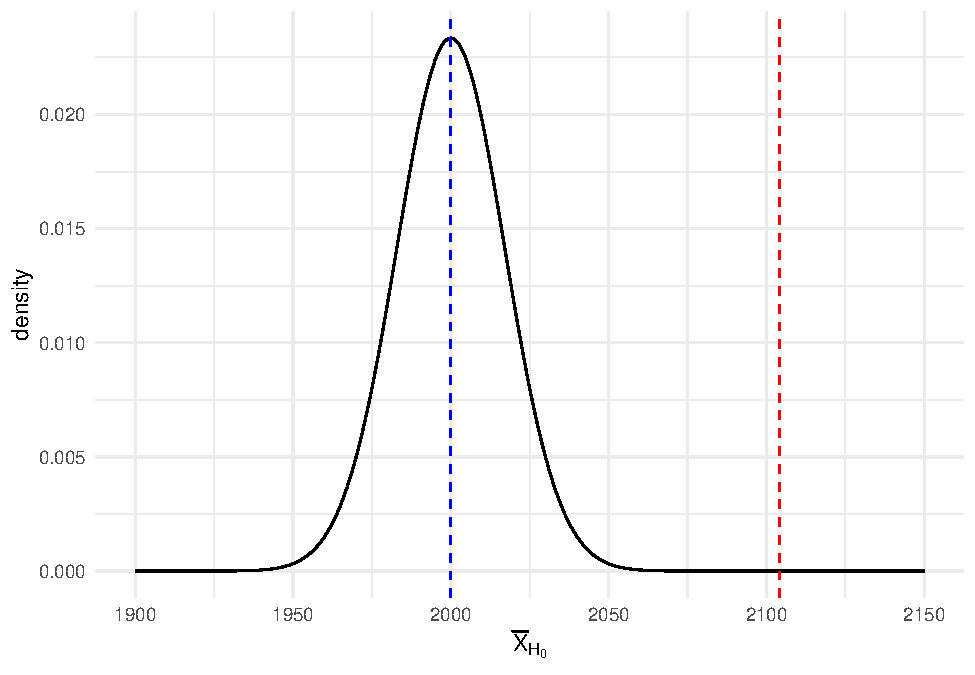
\includegraphics{Hypothesis_Testing_files/figure-latex/unnamed-chunk-5-1.pdf}
By using the distribution of the test statistic, it is possible to
identify a range of values that are unlikely to occur if \(H_0\) is
true. According to the significance level, we define a \textbf{critical
region}, values of the test the lead to the rejection of the null
hypothesis, and an \textbf{acceptance region}.\\
Suppose that we consider a significance level \(\alpha = 0.05\), the
critical region of a two-tailed test will corresponds to the most
extreme values (tails of the distribution). In this example

\begin{Shaded}
\begin{Highlighting}[]
\NormalTok{alpha }\OtherTok{\textless{}{-}} \FloatTok{0.05}
\NormalTok{quantiles }\OtherTok{\textless{}{-}} \FunctionTok{qnorm}\NormalTok{(}\FunctionTok{c}\NormalTok{(alpha}\SpecialCharTok{/}\DecValTok{2}\NormalTok{, }\DecValTok{1}\SpecialCharTok{{-}}\NormalTok{ alpha}\SpecialCharTok{/}\DecValTok{2}\NormalTok{), }
      \AttributeTok{mean =} \DecValTok{2000}\NormalTok{, }
      \AttributeTok{sd =}\NormalTok{ sd\_R}\SpecialCharTok{/}\FunctionTok{sqrt}\NormalTok{(n))}
\NormalTok{quantiles}
\end{Highlighting}
\end{Shaded}

\begin{verbatim}
## [1] 1966.511 2033.489
\end{verbatim}

\begin{Shaded}
\begin{Highlighting}[]
\FunctionTok{ggplot}\NormalTok{() }\SpecialCharTok{+} 
   \FunctionTok{geom\_line}\NormalTok{(}\AttributeTok{mapping =} \FunctionTok{aes}\NormalTok{(}\AttributeTok{x =}\NormalTok{ x, }\AttributeTok{y =}\NormalTok{ y)) }\SpecialCharTok{+} 
   \FunctionTok{theme\_minimal}\NormalTok{() }\SpecialCharTok{+} 
   \FunctionTok{geom\_vline}\NormalTok{(}\AttributeTok{xintercept =}\NormalTok{ mean\_R, }\AttributeTok{color =} \StringTok{"red"}\NormalTok{, }\AttributeTok{linetype =} \StringTok{"dashed"}\NormalTok{)  }\SpecialCharTok{+}
    \FunctionTok{xlab}\NormalTok{(}\FunctionTok{expression}\NormalTok{(}\FunctionTok{bar}\NormalTok{(X)[H[}\DecValTok{0}\NormalTok{]])) }\SpecialCharTok{+}
   \FunctionTok{ylab}\NormalTok{(}\StringTok{"density"}\NormalTok{)}\SpecialCharTok{+} 
   \FunctionTok{geom\_vline}\NormalTok{(}\AttributeTok{xintercept =}\NormalTok{ quantiles[}\DecValTok{1}\NormalTok{], }\AttributeTok{color =} \StringTok{"purple"}\NormalTok{, }\AttributeTok{linetype =} \StringTok{"dashed"}\NormalTok{)}\SpecialCharTok{+} 
   \FunctionTok{geom\_vline}\NormalTok{(}\AttributeTok{xintercept =}\NormalTok{ quantiles[}\DecValTok{2}\NormalTok{], }\AttributeTok{color =} \StringTok{"purple"}\NormalTok{, }\AttributeTok{linetype =} \StringTok{"dashed"}\NormalTok{)}
\end{Highlighting}
\end{Shaded}

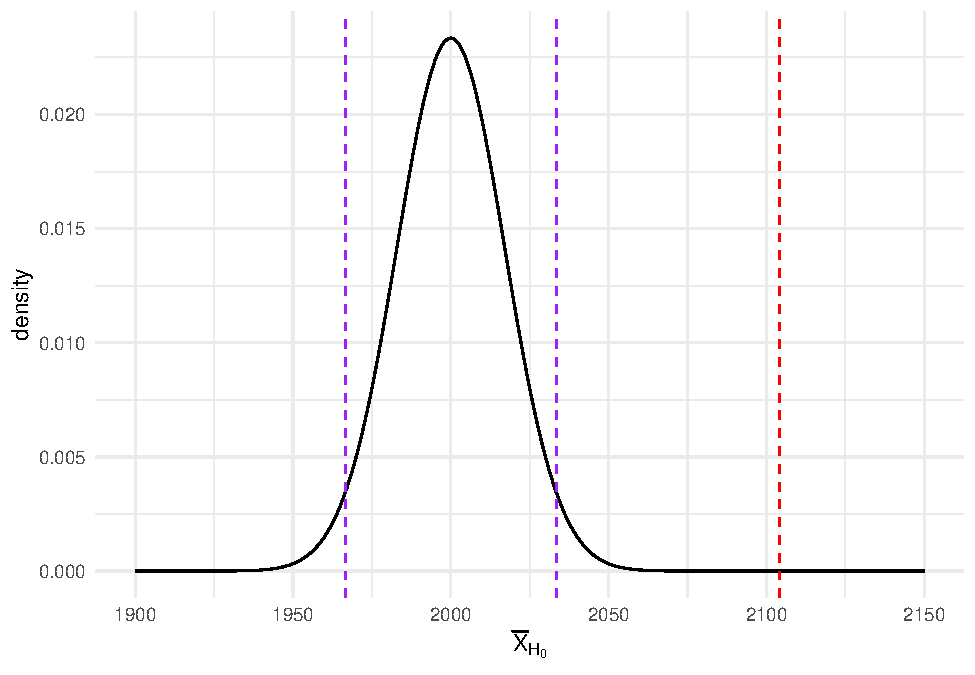
\includegraphics{Hypothesis_Testing_files/figure-latex/unnamed-chunk-6-1.pdf}
We can note that our statistic (sample mean) falls into the right
critical region, so we reject the null hypothesis. To sum up:

\begin{itemize}
\tightlist
\item
  choose an \(\alpha\) level,
\item
  come up with some test statistic that does a good job (in some
  meaningful sense),
\item
  figure out the sampling distribution of the test statistic on the
  assumption that the null hypothesis is true,
\item
  calculate the critical region that produces an appropriate \(\alpha\)
  level.
\end{itemize}

In addition we can compute the ``famous'' p-value. Note that a good
critical region almost always corresponds to those values of the test
statistic that are least likely to be observed if the null hypothesis is
true. Then the p-value can be defined as the probability that we would
have observed a test statistic that is at least as extreme as the one we
actually did get. In other words, if the data are extremely implausible
according to the null hypothesis, then the null hypothesis is probably
wrong.

\begin{Shaded}
\begin{Highlighting}[]
\DecValTok{2}\SpecialCharTok{*}\FunctionTok{pnorm}\NormalTok{(mean\_R, }
      \AttributeTok{mean =} \DecValTok{2000}\NormalTok{,}
      \AttributeTok{sd =}\NormalTok{ sd\_R}\SpecialCharTok{/}\FunctionTok{sqrt}\NormalTok{(n),}
      \AttributeTok{lower.tail =} \ConstantTok{FALSE}\NormalTok{)}
\end{Highlighting}
\end{Shaded}

\begin{verbatim}
## [1] 1.102789e-09
\end{verbatim}

The obtained value is very low, so we reject the null hypothesis.\\
\textbf{Remark}: the p-value is not the probability that the null
hypothesis is true or false.

In some circumstances, it is useful to consider \emph{one-tailed tests}
where the alternative hypothesis includes only one side of the value
specified in the null hypothesis. For example, in the study of the
response time assume that we are interested in showing some evidence
that the response time of the population under study is higher than the
average. Then we can consider
\[H_0: \mu = 2000 \mbox{ vs } H_1: \mu > 2000.\]

\begin{Shaded}
\begin{Highlighting}[]
\FunctionTok{t.test}\NormalTok{(dat}\SpecialCharTok{$}\NormalTok{Response\_Time, }\AttributeTok{mu=}\DecValTok{2000}\NormalTok{, }\AttributeTok{alternative=}\StringTok{"greater"}\NormalTok{)}
\end{Highlighting}
\end{Shaded}

\begin{verbatim}
## 
##  One Sample t-test
## 
## data:  dat$Response_Time
## t = 6.0938, df = 499, p-value = 1.104e-09
## alternative hypothesis: true mean is greater than 2000
## 95 percent confidence interval:
##  2075.963      Inf
## sample estimates:
## mean of x 
##   2104.12
\end{verbatim}

\hypertarget{then-h_0-is-not-rejected}{%
\subsubsection{\texorpdfstring{Then \(H_0\) is not
rejected}{Then H\_0 is not rejected}}\label{then-h_0-is-not-rejected}}

What is the meaning of not rejecting \(H_0\)? Unfortunately, we cannot
state that \(H_0\) is true, since ther is the possibility that the true
parameter is equal to a value very close to the tested value, or that
the result of the test depend on the low sample size. How do we
interpret the result?

\begin{itemize}
\tightlist
\item
  We can state that the data are compatible with the null hypothesis.
  There are no evidences that suggest to consider more complicated
  models for understanding the tested parameter.
\item
  The null hypothesis provide a conservative statement, while usually
  the alternative implies an effect, that is, the evidence are not so
  strong for rejecting \(H_0\).
\end{itemize}

\textbf{Remark}: Do not terminate a study with the results of a
hypothesis testing. In order to make inference on the population, it is
important to combine hypothesis testing with the results from the
estimation of parameters and confidence intervals. For example, if we
reject the null hypothesis but the confidence interval is large, then we
may not have enough information.

\hypertarget{example}{%
\paragraph{Example}\label{example}}

Let's consider an example where a metallurgical industry produces plates
with a thickness of \(14 \text{mm}\) and a tolerance of
\(0.5 \text{mm}\). Every shift (every 6 hours), 10 plates are sampled
and their thickness is measured.

\begin{Shaded}
\begin{Highlighting}[]
\NormalTok{thickness }\OtherTok{\textless{}{-}} \FunctionTok{c}\NormalTok{(}\FloatTok{13.88}\NormalTok{, }\FloatTok{14.03}\NormalTok{, }\FloatTok{14.11}\NormalTok{, }\FloatTok{13.77}\NormalTok{, }\FloatTok{14.04}\NormalTok{, }\FloatTok{14.05}\NormalTok{, }\FloatTok{13.94}\NormalTok{, }\FloatTok{13.95}\NormalTok{, }\FloatTok{13.94}\NormalTok{, }\FloatTok{13.91}\NormalTok{)}
\NormalTok{alpha }\OtherTok{\textless{}{-}} \FloatTok{0.05}
\NormalTok{Var }\OtherTok{\textless{}{-}} \FloatTok{0.01}
\NormalTok{x\_bar }\OtherTok{\textless{}{-}} \FunctionTok{mean}\NormalTok{(thickness)}
\NormalTok{n }\OtherTok{\textless{}{-}} \FunctionTok{length}\NormalTok{(thickness)}
\end{Highlighting}
\end{Shaded}

Consider that after each maintenance, the system is calibrated so that
the mean thickness of the plates is \(14 \text{mm}\). Therefore, a value
of \(\bar{X}\) different from this could indicate a malfunction. In this
case, it is useful to perform a hypothesis test considering
\(H_0: \mu = 14\) and \(H_1: \mu \neq 14\). If the null hypothesis is
verified, then it can be concluded (with a certain level of confidence)
that the system is functioning correctly. First, we calculate the test
statistic

\begin{Shaded}
\begin{Highlighting}[]
\NormalTok{mu0 }\OtherTok{\textless{}{-}} \DecValTok{14}
\NormalTok{sd\_thick }\OtherTok{\textless{}{-}} \FunctionTok{sd}\NormalTok{(thickness)}
\NormalTok{z\_oss }\OtherTok{\textless{}{-}}\NormalTok{ (x\_bar }\SpecialCharTok{{-}}\NormalTok{ mu0)}\SpecialCharTok{/}\NormalTok{(sd\_thick}\SpecialCharTok{/}\FunctionTok{sqrt}\NormalTok{(n))}
\end{Highlighting}
\end{Shaded}

We know that \(Z\) described above follows \(N(0,1)\). The considered
hypothesis test is a two-tailed test, so we can accept \(H_0\) with
confidence level \(\alpha\) if the observed value falls within the
\(\alpha\) confidence interval.

\begin{Shaded}
\begin{Highlighting}[]
\NormalTok{alpha }\OtherTok{\textless{}{-}} \FloatTok{0.05}
\NormalTok{interval }\OtherTok{\textless{}{-}} \FunctionTok{c}\NormalTok{(x\_bar }\SpecialCharTok{+} \FunctionTok{qt}\NormalTok{(alpha }\SpecialCharTok{/} \DecValTok{2}\NormalTok{, n}\DecValTok{{-}1}\NormalTok{)}\SpecialCharTok{*}\NormalTok{sd\_thick}\SpecialCharTok{/}\FunctionTok{sqrt}\NormalTok{(n), x\_bar }\SpecialCharTok{+} \FunctionTok{qt}\NormalTok{(}\DecValTok{1} \SpecialCharTok{{-}}\NormalTok{ alpha }\SpecialCharTok{/} \DecValTok{2}\NormalTok{, n}\DecValTok{{-}1}\NormalTok{)}\SpecialCharTok{*}\NormalTok{sd\_thick}\SpecialCharTok{/}\FunctionTok{sqrt}\NormalTok{(n))}
\NormalTok{interval}
\end{Highlighting}
\end{Shaded}

\begin{verbatim}
## [1] 13.89136 14.03264
\end{verbatim}

\begin{Shaded}
\begin{Highlighting}[]
\NormalTok{x\_bar}
\end{Highlighting}
\end{Shaded}

\begin{verbatim}
## [1] 13.962
\end{verbatim}

The true value is within the interval, so we cannot reject the null
hypothesis. Alternatively, we can calculate the \(p\)-value. In a
two-tailed hypothesis test, this is given by:

\begin{Shaded}
\begin{Highlighting}[]
\NormalTok{pval }\OtherTok{\textless{}{-}} \DecValTok{2}\SpecialCharTok{*}\FunctionTok{pt}\NormalTok{(z\_oss, }\AttributeTok{df=}\NormalTok{n}\DecValTok{{-}1}\NormalTok{)}
\NormalTok{pval}
\end{Highlighting}
\end{Shaded}

\begin{verbatim}
## [1] 0.2545875
\end{verbatim}

The \(p\)-value does not allow to reject the null hypothesis. The result
confirms that the system is functioning correctly for the considered
sample. We can do the same using the function \texttt{t.test}

\begin{Shaded}
\begin{Highlighting}[]
\FunctionTok{t.test}\NormalTok{(thickness, }\AttributeTok{mu =} \DecValTok{14}\NormalTok{)}
\end{Highlighting}
\end{Shaded}

\begin{verbatim}
## 
##  One Sample t-test
## 
## data:  thickness
## t = -1.2169, df = 9, p-value = 0.2546
## alternative hypothesis: true mean is not equal to 14
## 95 percent confidence interval:
##  13.89136 14.03264
## sample estimates:
## mean of x 
##    13.962
\end{verbatim}

Let us suppose we want to verify whether the system is currently
calibrated for thicknesses greater than \(14 \text{mm}\). In this case,
the null hypothesis is \(H_0: \mu = 14\) (equivalently \(\mu \leq 14\))
and \(H_1: \mu > 14\), or \(H_0: \mu = 14\) (equivalently
\(\mu \geq 14\)) and \(H_1: \mu < 14\). For example, in the first case:

\begin{Shaded}
\begin{Highlighting}[]
\NormalTok{pval }\OtherTok{\textless{}{-}} \FunctionTok{pt}\NormalTok{(z\_oss, }\AttributeTok{df=}\NormalTok{n}\DecValTok{{-}1}\NormalTok{)}
\NormalTok{pval}
\end{Highlighting}
\end{Shaded}

\begin{verbatim}
## [1] 0.1272937
\end{verbatim}

\hypertarget{example.}{%
\paragraph{Example.}\label{example.}}

A wholesale supplier of bathroom fixtures wants to maintain internal
control over sales. To do so, invoices must be accompanied by a transfer
receipt to remove goods from the warehouse. At the end of each month, a
sample of invoices is taken to evaluate the average amount reported.
Over the last 5 years, the average invoice amount has been \$120. Given
that transport costs are influenced by delivery distance, it is
important to monitor the average amount. Consider the following sample:

\begin{Shaded}
\begin{Highlighting}[]
\NormalTok{fatture }\OtherTok{\textless{}{-}} \FunctionTok{c}\NormalTok{(}\FloatTok{108.98}\NormalTok{, }\FloatTok{152.22}\NormalTok{, }\FloatTok{111.45}\NormalTok{, }\FloatTok{110.59}\NormalTok{, }\FloatTok{127.46}\NormalTok{, }\FloatTok{107.26}\NormalTok{, }\FloatTok{93.32}\NormalTok{, }
             \FloatTok{91.97}\NormalTok{, }\FloatTok{111.56}\NormalTok{, }\FloatTok{75.71}\NormalTok{, }\FloatTok{128.58}\NormalTok{, }\FloatTok{135.11}\NormalTok{)}
\NormalTok{mx }\OtherTok{\textless{}{-}} \FunctionTok{mean}\NormalTok{(fatture)}
\NormalTok{s2 }\OtherTok{\textless{}{-}} \FunctionTok{var}\NormalTok{(fatture)}
\end{Highlighting}
\end{Shaded}

We assume the distribution of the amounts, described by the random
variable \(X\), can be approximated by a normal distribution,
\(X \sim N(\mu_X, \sigma^2_X)\). We know that:
\[t = \sqrt{n}\frac{X - \bar{X}}{\sqrt{S^2}} \sim t_{n-1}\] follows a
\(t\)-distribution with \(n-1\) degrees of freedom. Next, we compare the
obtained sample mean with the known value \(\mu_0 = 120\). It is
appropriate to perform a two-tailed hypothesis test with
\(H_0: \mu = \mu_0\) and \(H_1: \mu \neq \mu_0\). We calculate the
observed \(t\)-value

\begin{Shaded}
\begin{Highlighting}[]
\NormalTok{n }\OtherTok{\textless{}{-}} \FunctionTok{length}\NormalTok{(fatture)}
\NormalTok{alpha }\OtherTok{\textless{}{-}} \FloatTok{0.01}
\NormalTok{z }\OtherTok{\textless{}{-}} \FunctionTok{qt}\NormalTok{(}\DecValTok{1} \SpecialCharTok{{-}}\NormalTok{ alpha }\SpecialCharTok{/} \DecValTok{2}\NormalTok{, n }\SpecialCharTok{{-}} \DecValTok{1}\NormalTok{)}
\NormalTok{interval }\OtherTok{\textless{}{-}} \FunctionTok{c}\NormalTok{(mx }\SpecialCharTok{{-}}\NormalTok{ z }\SpecialCharTok{*} \FunctionTok{sqrt}\NormalTok{(s2 }\SpecialCharTok{/}\NormalTok{ n), mx }\SpecialCharTok{+}\NormalTok{ z }\SpecialCharTok{*} \FunctionTok{sqrt}\NormalTok{(s2 }\SpecialCharTok{/}\NormalTok{ n))}
\NormalTok{interval}
\end{Highlighting}
\end{Shaded}

\begin{verbatim}
## [1]  94.2040 131.4977
\end{verbatim}

The value \(\mu_0\) is inside the 95\%-confidence interval. Equivalently
the interval of the test statistic

\begin{Shaded}
\begin{Highlighting}[]
\CommentTok{\# the interval of the test statistic}
\NormalTok{t\_oss }\OtherTok{\textless{}{-}}\NormalTok{ (mx }\SpecialCharTok{{-}} \DecValTok{120}\NormalTok{) }\SpecialCharTok{*} \FunctionTok{sqrt}\NormalTok{(n }\SpecialCharTok{/}\NormalTok{ s2)}
\NormalTok{t\_oss}
\end{Highlighting}
\end{Shaded}

\begin{verbatim}
## [1] -1.190761
\end{verbatim}

\begin{Shaded}
\begin{Highlighting}[]
\FunctionTok{c}\NormalTok{(z , z)}
\end{Highlighting}
\end{Shaded}

\begin{verbatim}
## [1] 3.105807 3.105807
\end{verbatim}

The statistic is inside the acceptance region. Alternatively we can
calculate the \(p\)-value

\begin{Shaded}
\begin{Highlighting}[]
\NormalTok{pval }\OtherTok{\textless{}{-}} \DecValTok{2} \SpecialCharTok{*} \FunctionTok{pt}\NormalTok{(}\SpecialCharTok{{-}}\NormalTok{t\_oss, n }\SpecialCharTok{{-}} \DecValTok{1}\NormalTok{, }\AttributeTok{lower.tail =} \ConstantTok{FALSE}\NormalTok{)}
\NormalTok{pval}
\end{Highlighting}
\end{Shaded}

\begin{verbatim}
## [1] 0.2588093
\end{verbatim}

Both results suggest that we fail to reject the null hypothesis. The
t.test function allows you to specify the type of test (two-tailed or
one-tailed) with the alternative argument.

\begin{Shaded}
\begin{Highlighting}[]
\CommentTok{\# Two{-}tailed test}
\FunctionTok{t.test}\NormalTok{(fatture, }\AttributeTok{mu =} \DecValTok{120}\NormalTok{, }\AttributeTok{conf.level =} \FloatTok{0.99}\NormalTok{)}
\end{Highlighting}
\end{Shaded}

\begin{verbatim}
## 
##  One Sample t-test
## 
## data:  fatture
## t = -1.1908, df = 11, p-value = 0.2588
## alternative hypothesis: true mean is not equal to 120
## 99 percent confidence interval:
##   94.2040 131.4977
## sample estimates:
## mean of x 
##  112.8508
\end{verbatim}

\begin{Shaded}
\begin{Highlighting}[]
\CommentTok{\# One{-}tailed tests}
\FunctionTok{t.test}\NormalTok{(fatture, }\AttributeTok{mu =} \DecValTok{120}\NormalTok{, }\AttributeTok{alternative =} \StringTok{"greater"}\NormalTok{, }\AttributeTok{conf.level =} \FloatTok{0.99}\NormalTok{)}
\end{Highlighting}
\end{Shaded}

\begin{verbatim}
## 
##  One Sample t-test
## 
## data:  fatture
## t = -1.1908, df = 11, p-value = 0.8706
## alternative hypothesis: true mean is greater than 120
## 99 percent confidence interval:
##  96.53186      Inf
## sample estimates:
## mean of x 
##  112.8508
\end{verbatim}

\begin{Shaded}
\begin{Highlighting}[]
\FunctionTok{t.test}\NormalTok{(fatture, }\AttributeTok{mu =} \DecValTok{120}\NormalTok{, }\AttributeTok{alternative =} \StringTok{"less"}\NormalTok{, }\AttributeTok{conf.level =} \FloatTok{0.99}\NormalTok{)}
\end{Highlighting}
\end{Shaded}

\begin{verbatim}
## 
##  One Sample t-test
## 
## data:  fatture
## t = -1.1908, df = 11, p-value = 0.1294
## alternative hypothesis: true mean is less than 120
## 99 percent confidence interval:
##      -Inf 129.1698
## sample estimates:
## mean of x 
##  112.8508
\end{verbatim}

In all cases, the confidence interval and \(p\)-value match the manually
computed values, confirming that the null hypothesis cannot be rejected.

\hypertarget{test-for-proportions}{%
\subsection{Test for Proportions}\label{test-for-proportions}}

Recall that, given the random variable \(X \sim Ber(p)\) and the sample
\(X_1, \ldots, X_n\) from \(X\), the sample mean or \emph{sample
proportion} represents the proportion of successes in the random
sample.\\
The sampling distribution of \(\hat{p}\) can be approximated by a Normal
distribution \[\hat{p} \approx N(p, p(1-p)/n)\] with \(n\) sufficiently
large.

Consider the variable \texttt{Sex} in the dat data set. We want to
compute the proportion of male, and then test is the sample proportion
is equal to the value 0.5. We can do this using the \texttt{prop.test}
function

\begin{Shaded}
\begin{Highlighting}[]
\FunctionTok{prop.test}\NormalTok{(}\FunctionTok{table}\NormalTok{(dat}\SpecialCharTok{$}\NormalTok{Sex), }\AttributeTok{conf.level =} \FloatTok{0.95}\NormalTok{, }\AttributeTok{alternative =} \StringTok{"less"}\NormalTok{)}
\end{Highlighting}
\end{Shaded}

\begin{verbatim}
## 
##  1-sample proportions test without continuity correction
## 
## data:  table(dat$Sex), null probability 0.5
## X-squared = 0, df = 1, p-value = 0.5
## alternative hypothesis: true p is less than 0.5
## 95 percent confidence interval:
##  0.0000000 0.5366809
## sample estimates:
##   p 
## 0.5
\end{verbatim}

\hypertarget{example-political-candidate}{%
\paragraph{Example: Political
Candidate}\label{example-political-candidate}}

A politician wants to run for office in a district with 100,000 voters.
Before announcing the candidacy, they want to assess their likelihood of
success. To do this, a survey company is hired to contact 2,500 voters.
Out of these, 1,328 declare themselves in favor of the candidate, which
corresponds to a percentage of:

\[
\frac{1328}{2500} \cdot 100\% = 53\%.
\]

We want to infer the unknown percentage \(p\) of voters favoring the
candidate. The assumptions are: - All respondents have the same
probability of being included in the sample. - Responses are independent
(no influence among respondents).

Under these conditions, the number of supporters \(y\) among the \(n\)
surveyed voters can be modeled as a random variable
\(Y \sim Bin(n, p)\). An estimate is given by:

\begin{Shaded}
\begin{Highlighting}[]
\NormalTok{n }\OtherTok{\textless{}{-}} \DecValTok{2500}
\NormalTok{y }\OtherTok{\textless{}{-}} \DecValTok{1328}
\NormalTok{p\_hat }\OtherTok{\textless{}{-}}\NormalTok{ y }\SpecialCharTok{/}\NormalTok{ n}
\NormalTok{p\_hat}
\end{Highlighting}
\end{Shaded}

\begin{verbatim}
## [1] 0.5312
\end{verbatim}

In general, the confidence interval is constructed using the normal
approximation \[\frac{\hat{p}-p}{\sqrt{p(1-p)}/\sqrt{n}} \sim N(0,1),\]
hence:

\begin{Shaded}
\begin{Highlighting}[]
\NormalTok{alpha }\OtherTok{\textless{}{-}} \FloatTok{0.1}
\NormalTok{Var }\OtherTok{\textless{}{-}}\NormalTok{ p\_hat }\SpecialCharTok{*}\NormalTok{ (}\DecValTok{1} \SpecialCharTok{{-}}\NormalTok{ p\_hat) }\SpecialCharTok{/}\NormalTok{ n}
\NormalTok{interval }\OtherTok{\textless{}{-}} \FunctionTok{c}\NormalTok{(p\_hat }\SpecialCharTok{{-}} \FunctionTok{qnorm}\NormalTok{(}\DecValTok{1} \SpecialCharTok{{-}}\NormalTok{ alpha }\SpecialCharTok{/} \DecValTok{2}\NormalTok{) }\SpecialCharTok{*} \FunctionTok{sqrt}\NormalTok{(Var), }
\NormalTok{              p\_hat }\SpecialCharTok{+} \FunctionTok{qnorm}\NormalTok{(}\DecValTok{1} \SpecialCharTok{{-}}\NormalTok{ alpha }\SpecialCharTok{/} \DecValTok{2}\NormalTok{) }\SpecialCharTok{*} \FunctionTok{sqrt}\NormalTok{(Var))}
\NormalTok{interval}
\end{Highlighting}
\end{Shaded}

\begin{verbatim}
## [1] 0.5147835 0.5476165
\end{verbatim}

Given this result, the politician may conclude that there is a
reasonable expectation of winning. It is also useful to perform a
hypothesis test with \(H_0: p = p_0\), where \(p_0 = 0.5\) (indifference
among voters), and \(H_1: p > p_0\)

\begin{Shaded}
\begin{Highlighting}[]
\NormalTok{p0 }\OtherTok{\textless{}{-}} \FloatTok{0.5}
\NormalTok{p\_hat}
\end{Highlighting}
\end{Shaded}

\begin{verbatim}
## [1] 0.5312
\end{verbatim}

\begin{Shaded}
\begin{Highlighting}[]
 \FunctionTok{c}\NormalTok{(}\SpecialCharTok{{-}}\ConstantTok{Inf}\NormalTok{, }
\NormalTok{  p0 }\SpecialCharTok{+} \FunctionTok{qnorm}\NormalTok{(}\DecValTok{1} \SpecialCharTok{{-}}\NormalTok{ alpha }\SpecialCharTok{/} \DecValTok{2}\NormalTok{) }\SpecialCharTok{*} \FunctionTok{sqrt}\NormalTok{(Var))}
\end{Highlighting}
\end{Shaded}

\begin{verbatim}
## [1]      -Inf 0.5164165
\end{verbatim}

The sample proportion is in the critical region. Alernatively, we can
compute the p-value

\begin{Shaded}
\begin{Highlighting}[]
\NormalTok{p\_obs }\OtherTok{\textless{}{-}}\NormalTok{ (p\_hat }\SpecialCharTok{{-}}\NormalTok{ p0) }\SpecialCharTok{/} \FunctionTok{sqrt}\NormalTok{(Var)}
\FunctionTok{pnorm}\NormalTok{(p\_obs, }\AttributeTok{lower.tail =} \ConstantTok{FALSE}\NormalTok{)}
\end{Highlighting}
\end{Shaded}

\begin{verbatim}
## [1] 0.0008857304
\end{verbatim}

Both results suggest rejecting the null hypothesis in favor of the
alternative hypothesis. The test can also be performed using an exact
binomial test with \texttt{binom.test} or using \texttt{prop.test},
which is based on the chi-squared distribution

\begin{Shaded}
\begin{Highlighting}[]
\FunctionTok{binom.test}\NormalTok{(y, n, }\AttributeTok{alternative =} \StringTok{"greater"}\NormalTok{, }\AttributeTok{conf.level =} \FloatTok{0.9}\NormalTok{)}
\end{Highlighting}
\end{Shaded}

\begin{verbatim}
## 
##  Exact binomial test
## 
## data:  y and n
## number of successes = 1328, number of trials = 2500, p-value =
## 0.0009647
## alternative hypothesis: true probability of success is greater than 0.5
## 90 percent confidence interval:
##  0.5181948 1.0000000
## sample estimates:
## probability of success 
##                 0.5312
\end{verbatim}

\begin{Shaded}
\begin{Highlighting}[]
\FunctionTok{prop.test}\NormalTok{(y, n, }\AttributeTok{correct =} \ConstantTok{FALSE}\NormalTok{, }\AttributeTok{alternative =} \StringTok{"greater"}\NormalTok{, }\AttributeTok{conf.level =} \FloatTok{0.9}\NormalTok{)}
\end{Highlighting}
\end{Shaded}

\begin{verbatim}
## 
##  1-sample proportions test without continuity correction
## 
## data:  y out of n, null probability 0.5
## X-squared = 9.7344, df = 1, p-value = 0.0009043
## alternative hypothesis: true p is greater than 0.5
## 90 percent confidence interval:
##  0.5183932 1.0000000
## sample estimates:
##      p 
## 0.5312
\end{verbatim}

\hypertarget{example-dr.-spock-and-the-jury-selection}{%
\paragraph{Example: Dr.~Spock and the Jury
Selection}\label{example-dr.-spock-and-the-jury-selection}}

Dr.~Benjamin Spock was a prominent pediatrician who, in 1968, was tried
in a federal court in Boston for conspiracy against the Military Service
Act due to his involvement in the anti-Vietnam War movement. The jury
selection raised controversy: only 102 out of 350 potential jurors were
women, even though 53\% of eligible voters were female.

The judge claimed the selection was random. Let us assess this claim
using a hypothesis test. Let \(N\) denote the total number of eligible
voters, and \(D\) the number of women among them. Under random
selection, the probability of choosing a woman in any draw is
\(p_0 = D/N\). Assuming \(N\) is large, this probability remains
approximately constant across selections. Thus, we can model \(X\), the
number of women among the selected jurors, as \(X \sim Bin(n,p)\), where
\(n\) is the number of selected jurors.

\begin{Shaded}
\begin{Highlighting}[]
\NormalTok{n }\OtherTok{\textless{}{-}} \DecValTok{350}
\NormalTok{d }\OtherTok{\textless{}{-}} \DecValTok{102}
\NormalTok{pn }\OtherTok{\textless{}{-}}\NormalTok{ d }\SpecialCharTok{/}\NormalTok{ n}
\NormalTok{pn}
\end{Highlighting}
\end{Shaded}

\begin{verbatim}
## [1] 0.2914286
\end{verbatim}

\begin{Shaded}
\begin{Highlighting}[]
\NormalTok{p0 }\OtherTok{\textless{}{-}} \FloatTok{0.53}
\end{Highlighting}
\end{Shaded}

We test \(H_0: p = p_0\) (the selection followed the law),
\(H_1: p\not=p_0\) (the selection was biased).We can use binom.test

\begin{Shaded}
\begin{Highlighting}[]
\FunctionTok{binom.test}\NormalTok{(d, n, p0)}
\end{Highlighting}
\end{Shaded}

\begin{verbatim}
## 
##  Exact binomial test
## 
## data:  d and n
## number of successes = 102, number of trials = 350, p-value < 2.2e-16
## alternative hypothesis: true probability of success is not equal to 0.53
## 95 percent confidence interval:
##  0.2443353 0.3420915
## sample estimates:
## probability of success 
##              0.2914286
\end{verbatim}

\begin{Shaded}
\begin{Highlighting}[]
\FunctionTok{prop.test}\NormalTok{(d, n, p0, }\AttributeTok{corr =} \ConstantTok{FALSE}\NormalTok{)}
\end{Highlighting}
\end{Shaded}

\begin{verbatim}
## 
##  1-sample proportions test without continuity correction
## 
## data:  d out of n, null probability p0
## X-squared = 79.971, df = 1, p-value < 2.2e-16
## alternative hypothesis: true p is not equal to 0.53
## 95 percent confidence interval:
##  0.2462908 0.3410950
## sample estimates:
##         p 
## 0.2914286
\end{verbatim}

In all cases, the obtained \(p\)-value is very low, suggesting rejection
of the null hypothesis. This indicates that it is difficult to believe
the jury selection was random.

\textbf{Conclusion of the Story}:\\
On July 10, 1968, Dr.~Spock was sentenced to two years in prison and
fined \$5,000. However, the verdict was overturned by the United States
Court of Appeals in 1969 due to insufficient evidence.

\hypertarget{comparison-of-means-of-two-normal-populations}{%
\subsection{Comparison of Means of Two Normal
Populations}\label{comparison-of-means-of-two-normal-populations}}

When the difference in population means is analyzed, we must think about
the type of sampling design we have:

\begin{enumerate}
\def\labelenumi{(\roman{enumi})}
\tightlist
\item
  Design with independent random samples,
\item
  Paired sampling design.
\end{enumerate}

These two sampling designs result in differences in the methods used to
compare the two populations.\\
Consider two independent random variables \(X_1\) and \(X_2\), and
corresponding samples of size \(n_1\) and \(n_2\), respectively. We
assume that \(X_1\sim N(\mu_1,\sigma_1)\) and
\(X_2\sim N(\mu_2,\sigma_2)\). To test whether \(\mu_1 > \mu_2\), we set
up the hypotheses \(H_0: \mu_1 = \mu_2\) vs \(H_1: \mu_1 > \mu_2\). This
is equivalent to:

\[H_0: \mu_1 - \mu_2 = 0 \quad \mbox{ vs } \mu_1 - \mu_2 > 0.\] Hence,
we can consider the results seen for testing the mean estimate of a
normally distributed random variable.

As in the case of a single mean \(\mu\), if we use an estimate of
\(\sigma^2_1\) and \(\sigma^2_2\) instead of the true population value
inside the confidence interval formulation, we must consider the
quantile of the student \(t\)-distribution instead of the standard
normal one. In this case the degrees of freedom \(df = n_1 + n_2 -2\)
for the first case, while the in the second case has a more complicated
formula that we will not consider here.

\hypertarget{example-wage-comparison-between-unionized-and-non-unionized-women}{%
\paragraph{Example: Wage Comparison Between Unionized and Non-Unionized
Women}\label{example-wage-comparison-between-unionized-and-non-unionized-women}}

The Wall Street Journal on July 26, 1994, stated:

\emph{``Women who are union members earn \$2.50 per hour more than women
who are not union members.''}

Based on this statement, it seems advantageous for women in the U.S. to
be part of a union. Suppose we have samples of wages for women who are
union members and those who are not:

\begin{Shaded}
\begin{Highlighting}[]
\NormalTok{iscritte }\OtherTok{\textless{}{-}} \FunctionTok{c}\NormalTok{(}\FloatTok{22.40}\NormalTok{, }\FloatTok{18.90}\NormalTok{, }\FloatTok{16.70}\NormalTok{, }\FloatTok{14.05}\NormalTok{, }\FloatTok{16.20}\NormalTok{, }\FloatTok{20.00}\NormalTok{, }\FloatTok{16.10}\NormalTok{, }\FloatTok{16.30}\NormalTok{, }\FloatTok{19.10}\NormalTok{, }\FloatTok{16.50}\NormalTok{, }\FloatTok{18.50}\NormalTok{, }\FloatTok{19.80}\NormalTok{, }\FloatTok{17.00}\NormalTok{, }\FloatTok{14.30}\NormalTok{, }\FloatTok{17.20}\NormalTok{)}
\NormalTok{non\_iscritte }\OtherTok{\textless{}{-}} \FunctionTok{c}\NormalTok{(}\FloatTok{17.60}\NormalTok{, }\FloatTok{14.40}\NormalTok{, }\FloatTok{16.60}\NormalTok{, }\FloatTok{15.00}\NormalTok{, }\FloatTok{17.65}\NormalTok{, }\FloatTok{15.00}\NormalTok{, }\FloatTok{17.55}\NormalTok{, }\FloatTok{13.30}\NormalTok{, }\FloatTok{11.20}\NormalTok{, }\FloatTok{15.90}\NormalTok{, }\FloatTok{19.20}\NormalTok{, }\FloatTok{11.85}\NormalTok{, }\FloatTok{16.65}\NormalTok{, }\FloatTok{15.20}\NormalTok{, }\FloatTok{15.30}\NormalTok{, }\FloatTok{17.00}\NormalTok{, }\FloatTok{15.10}\NormalTok{, }\FloatTok{14.30}\NormalTok{, }\FloatTok{13.90}\NormalTok{, }\FloatTok{14.50}\NormalTok{)}
\FunctionTok{length}\NormalTok{(iscritte)}
\end{Highlighting}
\end{Shaded}

\begin{verbatim}
## [1] 15
\end{verbatim}

\begin{Shaded}
\begin{Highlighting}[]
\FunctionTok{length}\NormalTok{(non\_iscritte)}
\end{Highlighting}
\end{Shaded}

\begin{verbatim}
## [1] 20
\end{verbatim}

We note that the two samples have different sizes. Descriptive
statistics and visualizations can be helpful for initial comparisons:

\begin{Shaded}
\begin{Highlighting}[]
\FunctionTok{boxplot}\NormalTok{(iscritte, non\_iscritte, }\AttributeTok{names =} \FunctionTok{c}\NormalTok{(}\StringTok{"Unionized"}\NormalTok{, }\StringTok{"Non{-}Unionized"}\NormalTok{))}
\end{Highlighting}
\end{Shaded}

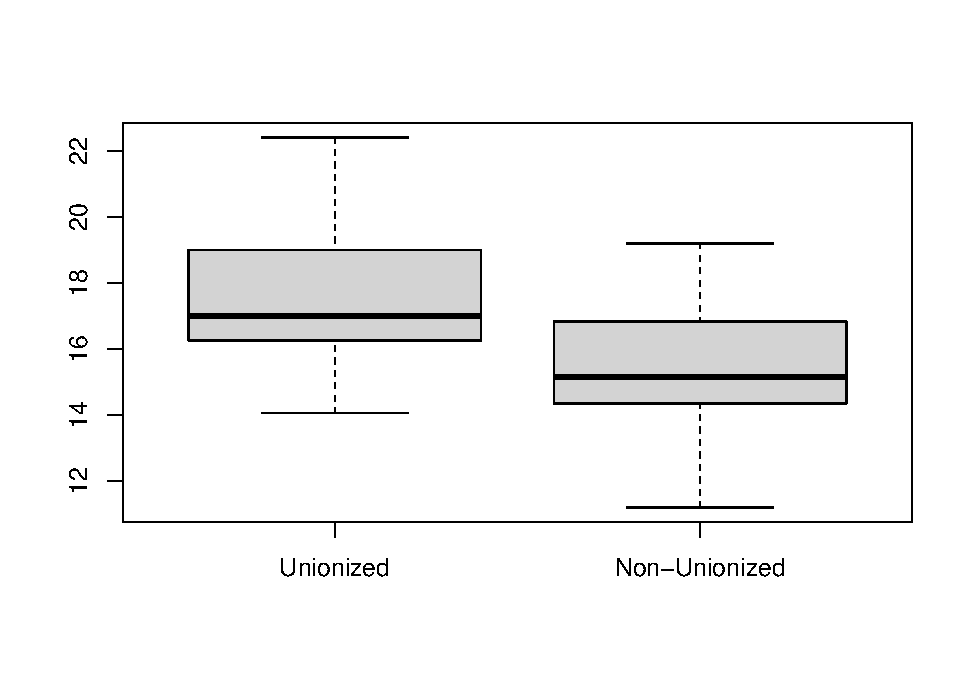
\includegraphics{Hypothesis_Testing_files/figure-latex/unnamed-chunk-29-1.pdf}

\begin{Shaded}
\begin{Highlighting}[]
\NormalTok{union\_dat }\OtherTok{\textless{}{-}} \FunctionTok{data.frame}\NormalTok{(}\AttributeTok{wages=}\FunctionTok{c}\NormalTok{(iscritte, non\_iscritte),}\AttributeTok{Union =} \FunctionTok{factor}\NormalTok{(}\FunctionTok{rep}\NormalTok{(}\FunctionTok{c}\NormalTok{(}\StringTok{"Unionized"}\NormalTok{, }\StringTok{"Non{-}Unionized"}\NormalTok{),}\AttributeTok{times=}\FunctionTok{c}\NormalTok{(}\FunctionTok{length}\NormalTok{(iscritte), }\FunctionTok{length}\NormalTok{(non\_iscritte)))))}
\FunctionTok{ggplot}\NormalTok{(union\_dat, }\FunctionTok{aes}\NormalTok{(}\AttributeTok{x =}\NormalTok{ Union, }\AttributeTok{y=}\NormalTok{wages, }\AttributeTok{fill=}\NormalTok{Union))}\SpecialCharTok{+}
  \FunctionTok{geom\_boxplot}\NormalTok{()}
\end{Highlighting}
\end{Shaded}

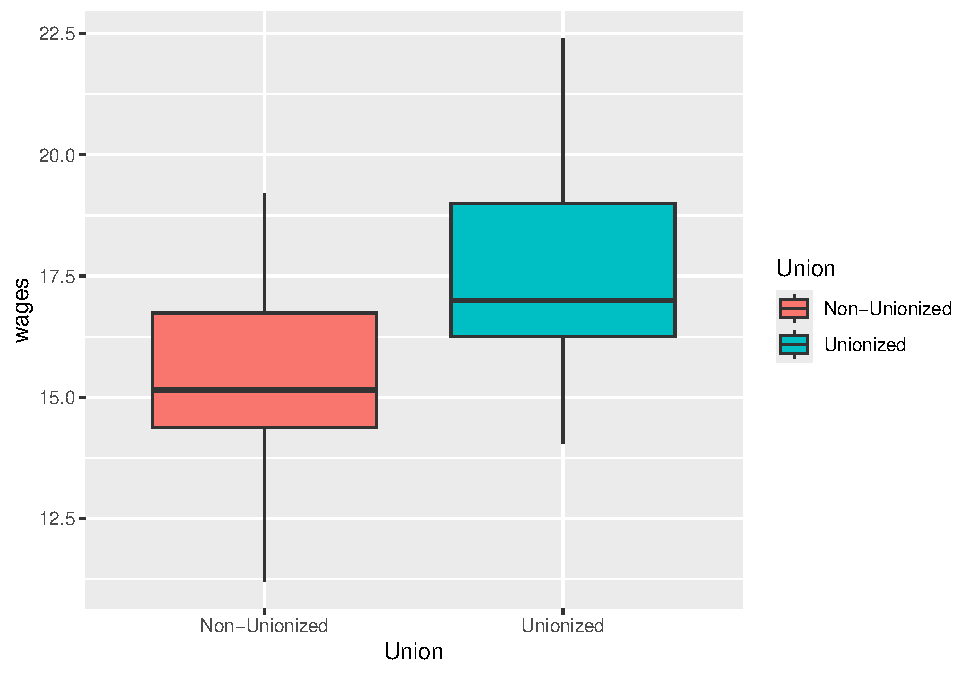
\includegraphics{Hypothesis_Testing_files/figure-latex/unnamed-chunk-29-2.pdf}

The boxplot comparison suggests that unionized women earn more on
average than non-unionized women, but this visualization does not
provide any measure of statistical significance or reliability.

Assume that the wages of both groups follow a normal distribution with
means \(\mu_1\) and \(\mu_2\), respectively, and the same variance
\(\sigma_1 = \sigma_2\). We also assume the two populations are
independent. The sample means are:

\begin{Shaded}
\begin{Highlighting}[]
\NormalTok{mu1 }\OtherTok{\textless{}{-}} \FunctionTok{mean}\NormalTok{(iscritte)}
\NormalTok{mu2 }\OtherTok{\textless{}{-}} \FunctionTok{mean}\NormalTok{(non\_iscritte)}
\FunctionTok{c}\NormalTok{(mu1, mu2)}
\end{Highlighting}
\end{Shaded}

\begin{verbatim}
## [1] 17.53667 15.36000
\end{verbatim}

To test whether \(\mu_1 > \mu_2\), we set up the following hypotheses:
\(H_0: \mu_1 = \mu_2\) vs \(H_1: \mu_1 > \mu_2\). This is equivalent to:

\[H_0: \mu_1 - \mu_2 = 0 \quad \mbox{ vs } \mu_1 - \mu_2 > 0.\] Since we
assume equal variances, we calculate the pooled variance:

\begin{Shaded}
\begin{Highlighting}[]
\NormalTok{s1 }\OtherTok{\textless{}{-}} \FunctionTok{var}\NormalTok{(iscritte)}
\NormalTok{s2 }\OtherTok{\textless{}{-}} \FunctionTok{var}\NormalTok{(non\_iscritte)}
\NormalTok{n }\OtherTok{\textless{}{-}} \FunctionTok{length}\NormalTok{(iscritte)}
\NormalTok{m }\OtherTok{\textless{}{-}} \FunctionTok{length}\NormalTok{(non\_iscritte)}
\NormalTok{s }\OtherTok{\textless{}{-}}\NormalTok{ ((n }\SpecialCharTok{{-}} \DecValTok{1}\NormalTok{) }\SpecialCharTok{*}\NormalTok{ s1 }\SpecialCharTok{+}\NormalTok{ (m }\SpecialCharTok{{-}} \DecValTok{1}\NormalTok{) }\SpecialCharTok{*}\NormalTok{ s2) }\SpecialCharTok{/}\NormalTok{ (n }\SpecialCharTok{+}\NormalTok{ m }\SpecialCharTok{{-}} \DecValTok{2}\NormalTok{)}
\end{Highlighting}
\end{Shaded}

The test statistic is given by:
\[t_{obs} = \frac{\bar{X}_1 - \bar{X}_1}{\sqrt{s(\frac{1}{n}+\frac{1}{m})}}.\]
Calculate the test statistic and \(p\)-value

\begin{Shaded}
\begin{Highlighting}[]
\NormalTok{mu1 }\SpecialCharTok{{-}}\NormalTok{ mu2}
\end{Highlighting}
\end{Shaded}

\begin{verbatim}
## [1] 2.176667
\end{verbatim}

\begin{Shaded}
\begin{Highlighting}[]
\NormalTok{alpha }\OtherTok{\textless{}{-}} \FloatTok{0.05}
\FunctionTok{c}\NormalTok{(}\SpecialCharTok{{-}}\ConstantTok{Inf}\NormalTok{, }\FunctionTok{qt}\NormalTok{(}\DecValTok{1} \SpecialCharTok{{-}}\NormalTok{ alpha, n }\SpecialCharTok{+}\NormalTok{ m }\SpecialCharTok{{-}} \DecValTok{2}\NormalTok{, }\AttributeTok{lower.tail =} \ConstantTok{FALSE}\NormalTok{)}\SpecialCharTok{*} \FunctionTok{sqrt}\NormalTok{(s }\SpecialCharTok{*}\NormalTok{ (}\DecValTok{1} \SpecialCharTok{/}\NormalTok{ n }\SpecialCharTok{+} \DecValTok{1} \SpecialCharTok{/}\NormalTok{ m)))}
\end{Highlighting}
\end{Shaded}

\begin{verbatim}
## [1]      -Inf -1.213325
\end{verbatim}

\begin{Shaded}
\begin{Highlighting}[]
\CommentTok{\# Or computing the p{-}value}
\NormalTok{t\_obs }\OtherTok{\textless{}{-}}\NormalTok{ (mu1 }\SpecialCharTok{{-}}\NormalTok{ mu2) }\SpecialCharTok{/} \FunctionTok{sqrt}\NormalTok{(s }\SpecialCharTok{*}\NormalTok{ (}\DecValTok{1} \SpecialCharTok{/}\NormalTok{ n }\SpecialCharTok{+} \DecValTok{1} \SpecialCharTok{/}\NormalTok{ m))}
\FunctionTok{pt}\NormalTok{(t\_obs, n }\SpecialCharTok{+}\NormalTok{ m }\SpecialCharTok{{-}} \DecValTok{2}\NormalTok{, }\AttributeTok{lower.tail =} \ConstantTok{FALSE}\NormalTok{)}
\end{Highlighting}
\end{Shaded}

\begin{verbatim}
## [1] 0.002327084
\end{verbatim}

Alternatively, use the built-in t-test function:

\begin{Shaded}
\begin{Highlighting}[]
\FunctionTok{t.test}\NormalTok{(iscritte, non\_iscritte, }\AttributeTok{alternative =} \StringTok{"greater"}\NormalTok{, }\AttributeTok{var.equal =} \ConstantTok{TRUE}\NormalTok{)}
\end{Highlighting}
\end{Shaded}

\begin{verbatim}
## 
##  Two Sample t-test
## 
## data:  iscritte and non_iscritte
## t = 3.036, df = 33, p-value = 0.002327
## alternative hypothesis: true difference in means is greater than 0
## 95 percent confidence interval:
##  0.963342      Inf
## sample estimates:
## mean of x mean of y 
##  17.53667  15.36000
\end{verbatim}

The test suggests rejecting the null hypothesis in favor of the
alternative. The confidence interval for the difference in means did not
include 0, supporting the conclusion that unionized women earn
significantly more than non-unionized women, on average.

\textbf{Remark}: Notice that in this case we are assuming that the two
populations have equal variance. In case the sample sizes are large, the
t-test still works even if the standard deviations differ up to 3 times.
If this difference is larger than 3 times, or the groups are unbalanced
(the sample sizes are very different), the \(t\) test should not be
used. In the case of different variances, we can perform the \(t\) test
with the Welch approximation.

\hypertarget{paired-samples}{%
\paragraph{Paired samples}\label{paired-samples}}

Let's now see the last case, i.e., we have a paired sampling design.

Given \(X_1 \sim N(\mu_1,\sigma^2_1)\) and
\(X_2\sim N(\mu_2,\sigma^2_2)\), when paired sampling is used, we We can
consider \[D = X_1- X_2 \sim N(\mu_1- \mu_2,\sigma^2_{X_1 -X_2}).\]

For example, considering the data set \texttt{dat} previously loaded, we
can compare the Response\_Time collected in occasion 0 and occasion 1.
This data are paired, since they refer to the same observation.

\begin{Shaded}
\begin{Highlighting}[]
\FunctionTok{t.test}\NormalTok{(dat}\SpecialCharTok{$}\NormalTok{Response\_Time[}\FunctionTok{which}\NormalTok{(dat}\SpecialCharTok{$}\NormalTok{Time}\SpecialCharTok{==}\DecValTok{1} \SpecialCharTok{\&}\NormalTok{ dat}\SpecialCharTok{$}\NormalTok{Group}\SpecialCharTok{==}\StringTok{"Control"}\NormalTok{)],}
\NormalTok{       dat}\SpecialCharTok{$}\NormalTok{Response\_Time[}\FunctionTok{which}\NormalTok{(dat}\SpecialCharTok{$}\NormalTok{Time}\SpecialCharTok{==}\DecValTok{2}\SpecialCharTok{\&}\NormalTok{ dat}\SpecialCharTok{$}\NormalTok{Group}\SpecialCharTok{==}\StringTok{"Control"}\NormalTok{)], }
       \AttributeTok{conf.level =} \FloatTok{0.95}\NormalTok{,}
       \AttributeTok{var.equal =} \ConstantTok{FALSE}\NormalTok{,}
       \AttributeTok{paired =} \ConstantTok{TRUE}\NormalTok{)}
\end{Highlighting}
\end{Shaded}

\begin{verbatim}
## 
##  Paired t-test
## 
## data:  dat$Response_Time[which(dat$Time == 1 & dat$Group == "Control")] and dat$Response_Time[which(dat$Time == 2 & dat$Group == "Control")]
## t = -12.353, df = 24, p-value = 6.847e-12
## alternative hypothesis: true mean difference is not equal to 0
## 95 percent confidence interval:
##  -238.4414 -170.1697
## sample estimates:
## mean difference 
##       -204.3055
\end{verbatim}

\hypertarget{comparison-of-variances}{%
\subsection{Comparison of Variances}\label{comparison-of-variances}}

Consider the following simulated data:

\begin{Shaded}
\begin{Highlighting}[]
\NormalTok{n }\OtherTok{\textless{}{-}} \DecValTok{38}
\NormalTok{m }\OtherTok{\textless{}{-}} \DecValTok{50}
\NormalTok{x }\OtherTok{\textless{}{-}} \FunctionTok{rnorm}\NormalTok{(n, }\AttributeTok{sd =} \DecValTok{5}\NormalTok{)}
\NormalTok{y }\OtherTok{\textless{}{-}} \FunctionTok{rnorm}\NormalTok{(m, }\AttributeTok{sd =} \DecValTok{3}\NormalTok{)}
\NormalTok{s2x }\OtherTok{\textless{}{-}} \FunctionTok{var}\NormalTok{(x)}
\NormalTok{s2y }\OtherTok{\textless{}{-}} \FunctionTok{var}\NormalTok{(y)}
\FunctionTok{c}\NormalTok{(s2x, s2y)}
\end{Highlighting}
\end{Shaded}

\begin{verbatim}
## [1] 26.046961  8.045141
\end{verbatim}

Suppose \(X \sim N(\mu_x, \sigma^2_x)\) and
\(Y \sim N(\mu_y, \sigma^2_y)\). In this example, we are interested in
comparing the variability of the two datasets. After calculating the
sample variances, we want to perform the following hypothesis test \[
\begin{cases}
H_0: \sigma_x^2 = \sigma_y^2 \\
H_1: \sigma_x^2 \neq \sigma_y^2
\end{cases}
\] Since variances are strictly greater than zero, we focus on the ratio
\(\sigma_x^2 / \sigma_y^2\). Under the null hypothesis
\(\sigma_x^2 = \sigma_y^2\), we know \[
\frac{(n-1)s_x^2}{\sigma_x^2} \sim \chi^2_{n-1}, \quad 
\frac{(m-1)s_y^2}{\sigma_y^2} \sim \chi^2_{m-1}.
\] Thus, under \(H_0\), the ratio of variances follows an
\(F\)-distribution \[
\frac{s_x^2}{s_y^2} \sim F(n-1, m-1).
\] The confidence interval for the variance ratio is calculated as

\begin{Shaded}
\begin{Highlighting}[]
\NormalTok{s2x }\SpecialCharTok{/}\NormalTok{ s2y}
\end{Highlighting}
\end{Shaded}

\begin{verbatim}
## [1] 3.237602
\end{verbatim}

\begin{Shaded}
\begin{Highlighting}[]
\NormalTok{alpha }\OtherTok{\textless{}{-}} \FloatTok{0.05}
\NormalTok{interval }\OtherTok{\textless{}{-}} \FunctionTok{c}\NormalTok{(}
\NormalTok{  (s2x }\SpecialCharTok{/}\NormalTok{ s2y) }\SpecialCharTok{/} \FunctionTok{qf}\NormalTok{(}\DecValTok{1} \SpecialCharTok{{-}}\NormalTok{ alpha }\SpecialCharTok{/} \DecValTok{2}\NormalTok{, n }\SpecialCharTok{{-}} \DecValTok{1}\NormalTok{, m }\SpecialCharTok{{-}} \DecValTok{1}\NormalTok{),}
\NormalTok{  (s2x }\SpecialCharTok{/}\NormalTok{ s2y) }\SpecialCharTok{/} \FunctionTok{qf}\NormalTok{(alpha }\SpecialCharTok{/} \DecValTok{2}\NormalTok{, n }\SpecialCharTok{{-}} \DecValTok{1}\NormalTok{, m }\SpecialCharTok{{-}} \DecValTok{1}\NormalTok{)}
\NormalTok{)}
\NormalTok{interval}
\end{Highlighting}
\end{Shaded}

\begin{verbatim}
## [1] 1.778867 6.050048
\end{verbatim}

We can perform an \(F\)-test using the \texttt{var.test} function

\begin{Shaded}
\begin{Highlighting}[]
\FunctionTok{var.test}\NormalTok{(x, y)}
\end{Highlighting}
\end{Shaded}

\begin{verbatim}
## 
##  F test to compare two variances
## 
## data:  x and y
## F = 3.2376, num df = 37, denom df = 49, p-value = 0.0001428
## alternative hypothesis: true ratio of variances is not equal to 1
## 95 percent confidence interval:
##  1.778867 6.050048
## sample estimates:
## ratio of variances 
##           3.237602
\end{verbatim}

For a one-sided test to check if \(\sigma_x^2 > \sigma_y^2\), specify
the alternative hypothesis

\begin{Shaded}
\begin{Highlighting}[]
\FunctionTok{var.test}\NormalTok{(x, y, }\AttributeTok{alternative =} \StringTok{"greater"}\NormalTok{)}
\end{Highlighting}
\end{Shaded}

\begin{verbatim}
## 
##  F test to compare two variances
## 
## data:  x and y
## F = 3.2376, num df = 37, denom df = 49, p-value = 7.139e-05
## alternative hypothesis: true ratio of variances is greater than 1
## 95 percent confidence interval:
##  1.959994      Inf
## sample estimates:
## ratio of variances 
##           3.237602
\end{verbatim}

The \(F\)-test results include:

\begin{itemize}
\tightlist
\item
  Test statistic (F): The ratio of variances.
\item
  Degrees of freedom: \(n - 1\) and \(m - 1\) for the numerator and
  denominator.
\item
  \(p\)-value: Indicates the strength of evidence against \(H_0\).
\end{itemize}

\hypertarget{comparison-of-two-proportions}{%
\subsection{Comparison of two
Proportions}\label{comparison-of-two-proportions}}

Consider the following data, representing the number of graduates in
2001 in Economics at Ca' Foscari and Bocconi. The graduates are
classified based on the time elapsed between graduation and their first
job.

\begin{Shaded}
\begin{Highlighting}[]
\NormalTok{laureati }\OtherTok{\textless{}{-}} \FunctionTok{data.frame}\NormalTok{(}\AttributeTok{Ca.Foscari =} \FunctionTok{c}\NormalTok{(}\DecValTok{480}\NormalTok{, }\DecValTok{129}\NormalTok{), }\AttributeTok{Bocconi =} \FunctionTok{c}\NormalTok{(}\DecValTok{1338}\NormalTok{, }\DecValTok{438}\NormalTok{))}
\FunctionTok{rownames}\NormalTok{(laureati) }\OtherTok{\textless{}{-}} \FunctionTok{c}\NormalTok{(}\StringTok{"meno di un anno"}\NormalTok{, }\StringTok{"piu\textquotesingle{} di un anno"}\NormalTok{)}
\NormalTok{laureati}
\end{Highlighting}
\end{Shaded}

\begin{verbatim}
##                 Ca.Foscari Bocconi
## meno di un anno        480    1338
## piu' di un anno        129     438
\end{verbatim}

We add the total number of graduates for both universities and each
category to the table.

\begin{Shaded}
\begin{Highlighting}[]
\NormalTok{laureati}\SpecialCharTok{$}\NormalTok{Totale }\OtherTok{\textless{}{-}}\NormalTok{ laureati}\SpecialCharTok{$}\NormalTok{Ca.Foscari }\SpecialCharTok{+}\NormalTok{ laureati}\SpecialCharTok{$}\NormalTok{Bocconi}
\FunctionTok{rbind}\NormalTok{(laureati, }\FunctionTok{apply}\NormalTok{(laureati, }\DecValTok{2}\NormalTok{, sum))}
\end{Highlighting}
\end{Shaded}

\begin{verbatim}
##                 Ca.Foscari Bocconi Totale
## meno di un anno        480    1338   1818
## piu' di un anno        129     438    567
## 3                      609    1776   2385
\end{verbatim}

The event of interest is finding a job after graduation. Based on the
available information, we can assume that the random variable describing
this event follows a binomial distribution, where success corresponds to
finding a job within a year of graduation. First, we calculate the
empirical success probabilities for each university.

\begin{Shaded}
\begin{Highlighting}[]
\NormalTok{n1 }\OtherTok{\textless{}{-}} \FunctionTok{sum}\NormalTok{(laureati}\SpecialCharTok{$}\NormalTok{Ca.Foscari)}
\NormalTok{prop1 }\OtherTok{\textless{}{-}}\NormalTok{ laureati}\SpecialCharTok{$}\NormalTok{Ca.Foscari }\SpecialCharTok{/}\NormalTok{ n1}
\NormalTok{prop1}
\end{Highlighting}
\end{Shaded}

\begin{verbatim}
## [1] 0.7881773 0.2118227
\end{verbatim}

\begin{Shaded}
\begin{Highlighting}[]
\NormalTok{n2 }\OtherTok{\textless{}{-}} \FunctionTok{sum}\NormalTok{(laureati}\SpecialCharTok{$}\NormalTok{Bocconi)}
\NormalTok{prop2 }\OtherTok{\textless{}{-}}\NormalTok{ laureati}\SpecialCharTok{$}\NormalTok{Bocconi }\SpecialCharTok{/}\NormalTok{ n2}
\NormalTok{prop2}
\end{Highlighting}
\end{Shaded}

\begin{verbatim}
## [1] 0.7533784 0.2466216
\end{verbatim}

It is helpful to represent this data visually using bar plots to compare
the quantities. For instance

\begin{Shaded}
\begin{Highlighting}[]
\FunctionTok{barplot}\NormalTok{(}\FunctionTok{as.matrix}\NormalTok{(laureati[, }\SpecialCharTok{{-}}\DecValTok{3}\NormalTok{]), }\AttributeTok{legend.text =} \FunctionTok{c}\NormalTok{(}\StringTok{"meno di un anno"}\NormalTok{, }\StringTok{"piu\textquotesingle{} di un anno"}\NormalTok{))}
\end{Highlighting}
\end{Shaded}

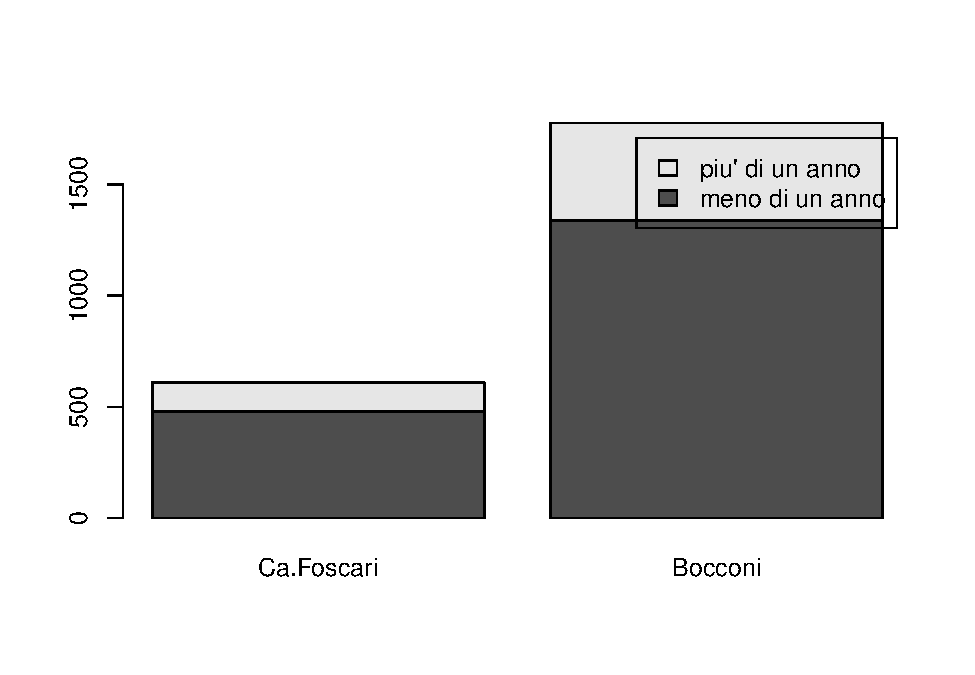
\includegraphics{Hypothesis_Testing_files/figure-latex/unnamed-chunk-42-1.pdf}

\begin{Shaded}
\begin{Highlighting}[]
\NormalTok{laureati}\SpecialCharTok{$}\NormalTok{Category }\OtherTok{\textless{}{-}} \FunctionTok{rownames}\NormalTok{(laureati)}
\NormalTok{laureati\_long }\OtherTok{\textless{}{-}} \FunctionTok{pivot\_longer}\NormalTok{(laureati, }\AttributeTok{cols =} \FunctionTok{c}\NormalTok{(}\StringTok{"Ca.Foscari"}\NormalTok{, }\StringTok{"Bocconi"}\NormalTok{), }\AttributeTok{names\_to =} \StringTok{"University"}\NormalTok{, }\AttributeTok{values\_to =} \StringTok{"Count"}\NormalTok{)}

\CommentTok{\# Generate the bar plot}
\FunctionTok{ggplot}\NormalTok{(laureati\_long, }\FunctionTok{aes}\NormalTok{(}\AttributeTok{x =}\NormalTok{ Category, }\AttributeTok{y =}\NormalTok{ Count, }\AttributeTok{fill =}\NormalTok{ University)) }\SpecialCharTok{+}
  \FunctionTok{geom\_bar}\NormalTok{(}\AttributeTok{stat =} \StringTok{"identity"}\NormalTok{, }\AttributeTok{position =} \StringTok{"dodge"}\NormalTok{) }\SpecialCharTok{+}
  \FunctionTok{labs}\NormalTok{(}
    \AttributeTok{title =} \StringTok{"Comparison of Graduates by University and Time to Find a Job"}\NormalTok{,}
    \AttributeTok{x =} \StringTok{"Time to Find a Job"}\NormalTok{,}
    \AttributeTok{y =} \StringTok{"Number of Graduates"}\NormalTok{,}
    \AttributeTok{fill =} \StringTok{"University"}
\NormalTok{  ) }\SpecialCharTok{+}
  \FunctionTok{theme\_minimal}\NormalTok{()}
\end{Highlighting}
\end{Shaded}

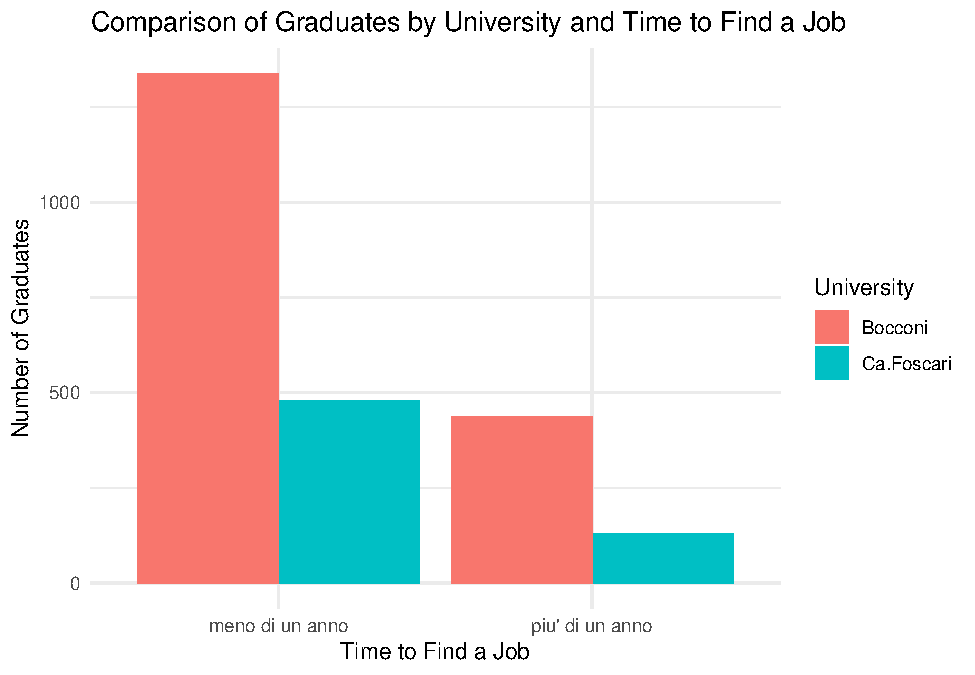
\includegraphics{Hypothesis_Testing_files/figure-latex/unnamed-chunk-42-2.pdf}

This plot is not very informative due to the difference in total
graduates between the two universities. It is more useful to represent
the proportions

\begin{Shaded}
\begin{Highlighting}[]
\FunctionTok{barplot}\NormalTok{(}\FunctionTok{cbind}\NormalTok{(prop1, prop2), }\AttributeTok{beside =} \ConstantTok{TRUE}\NormalTok{, }\AttributeTok{ylim =} \FunctionTok{c}\NormalTok{(}\DecValTok{0}\NormalTok{, }\DecValTok{1}\NormalTok{),}
       \AttributeTok{legend.text =} \FunctionTok{c}\NormalTok{(}\StringTok{"meno di un anno"}\NormalTok{, }\StringTok{"piu\textquotesingle{} di un anno"}\NormalTok{),}
       \AttributeTok{names.arg =} \FunctionTok{c}\NormalTok{(}\StringTok{"Ca\textquotesingle{} Foscari"}\NormalTok{, }\StringTok{"Bocconi"}\NormalTok{))}
\end{Highlighting}
\end{Shaded}

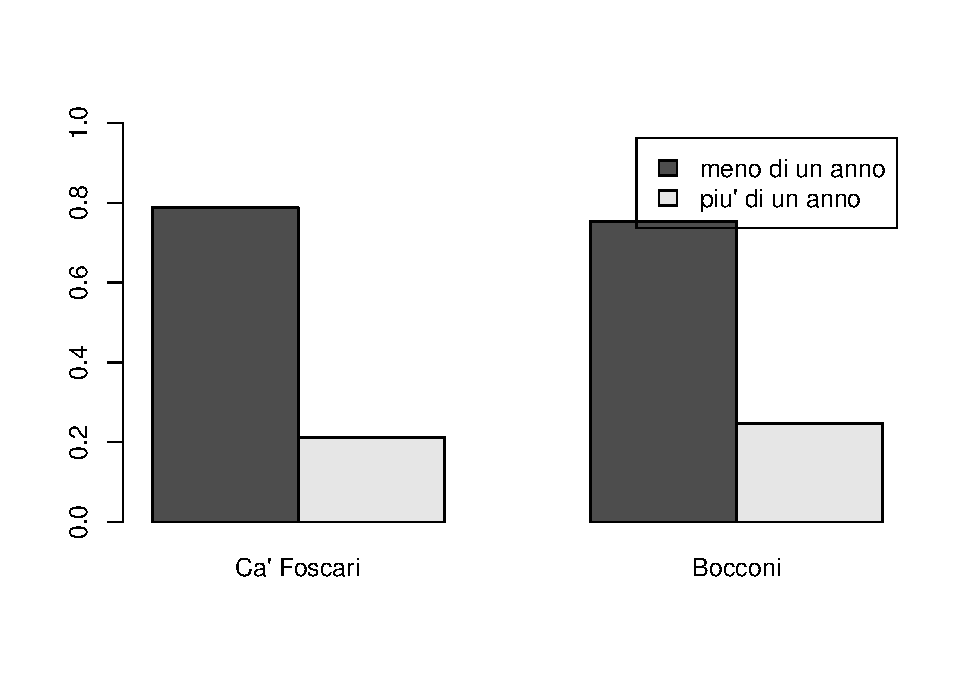
\includegraphics{Hypothesis_Testing_files/figure-latex/unnamed-chunk-43-1.pdf}
Note that the \emph{beside} option creates subgroups.

\begin{Shaded}
\begin{Highlighting}[]
\CommentTok{\# Calculate proportions for each university}
\NormalTok{laureati }\OtherTok{\textless{}{-}}\NormalTok{ laureati }\SpecialCharTok{\%\textgreater{}\%}
  \FunctionTok{mutate}\NormalTok{(}
    \AttributeTok{Prop\_Ca\_Foscari =}\NormalTok{ Ca.Foscari }\SpecialCharTok{/}\NormalTok{ Totale,}
    \AttributeTok{Prop\_Bocconi =}\NormalTok{ Bocconi }\SpecialCharTok{/}\NormalTok{ Totale}
\NormalTok{  )}

\CommentTok{\# Reshape the data to long format for ggplot}
\NormalTok{laureati\_long }\OtherTok{\textless{}{-}}\NormalTok{ laureati }\SpecialCharTok{\%\textgreater{}\%}
  \FunctionTok{select}\NormalTok{(Category, Prop\_Ca\_Foscari, Prop\_Bocconi) }\SpecialCharTok{\%\textgreater{}\%}
  \FunctionTok{pivot\_longer}\NormalTok{(}\AttributeTok{cols =} \FunctionTok{c}\NormalTok{(}\StringTok{"Prop\_Ca\_Foscari"}\NormalTok{, }\StringTok{"Prop\_Bocconi"}\NormalTok{), }
               \AttributeTok{names\_to =} \StringTok{"University"}\NormalTok{, }
               \AttributeTok{values\_to =} \StringTok{"Proportion"}\NormalTok{) }\SpecialCharTok{\%\textgreater{}\%}
  \FunctionTok{mutate}\NormalTok{(}\AttributeTok{University =} \FunctionTok{recode}\NormalTok{(University, }
                             \StringTok{"Prop\_Ca\_Foscari"} \OtherTok{=} \StringTok{"Ca\textquotesingle{} Foscari"}\NormalTok{, }
                             \StringTok{"Prop\_Bocconi"} \OtherTok{=} \StringTok{"Bocconi"}\NormalTok{))}

\CommentTok{\# Generate the bar plot}
\FunctionTok{ggplot}\NormalTok{(laureati\_long, }\FunctionTok{aes}\NormalTok{(}\AttributeTok{x =}\NormalTok{ Category, }\AttributeTok{y =}\NormalTok{ Proportion, }\AttributeTok{fill =}\NormalTok{ University)) }\SpecialCharTok{+}
  \FunctionTok{geom\_bar}\NormalTok{(}\AttributeTok{stat =} \StringTok{"identity"}\NormalTok{, }\AttributeTok{position =} \StringTok{"dodge"}\NormalTok{) }\SpecialCharTok{+}
  \FunctionTok{scale\_y\_continuous}\NormalTok{(}\AttributeTok{labels =}\NormalTok{ scales}\SpecialCharTok{::}\NormalTok{percent) }\SpecialCharTok{+} \CommentTok{\# Display proportions as percentages}
  \FunctionTok{labs}\NormalTok{(}
    \AttributeTok{title =} \StringTok{"Proportion of Graduates by University and Time to Find a Job"}\NormalTok{,}
    \AttributeTok{x =} \StringTok{"Time to Find a Job"}\NormalTok{,}
    \AttributeTok{y =} \StringTok{"Proportion of Graduates"}\NormalTok{,}
    \AttributeTok{fill =} \StringTok{"University"}
\NormalTok{  ) }\SpecialCharTok{+}
  \FunctionTok{theme\_minimal}\NormalTok{()}
\end{Highlighting}
\end{Shaded}

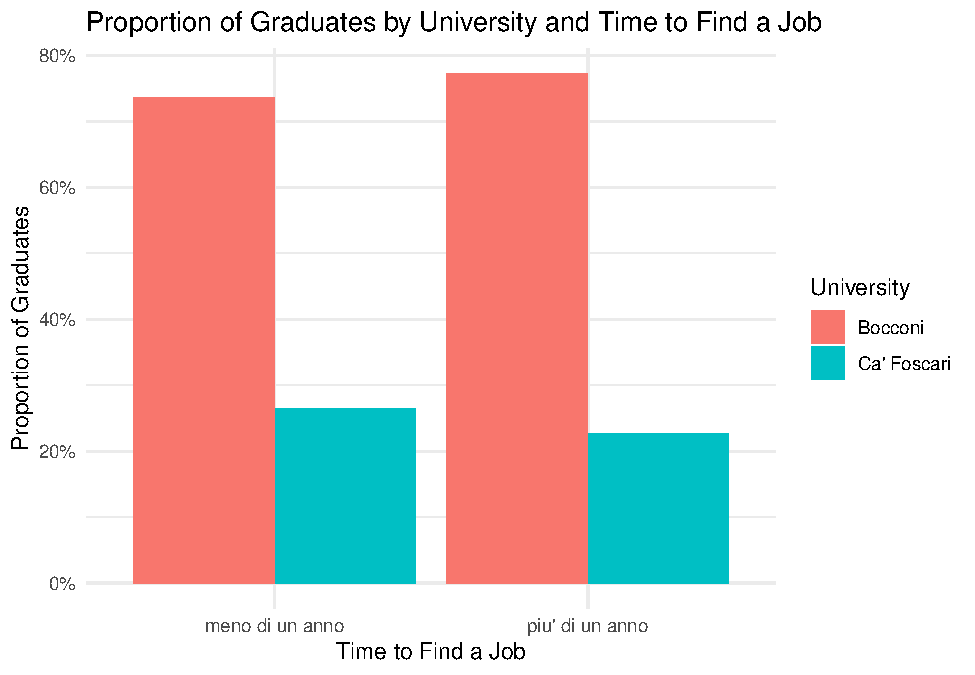
\includegraphics{Hypothesis_Testing_files/figure-latex/unnamed-chunk-44-1.pdf}

The statistics suggest that graduates from Ca' Foscari find jobs more
quickly. To assess the reliability of this result based on the sample
data, we can use confidence intervals and hypothesis tests. Let
\(Y_1 \sim \text{Bin}(n_1, p_1)\) and \(Y_2 \sim \text{Bin}(n_2, p_2)\)
be independent random variables describing the number of graduates at
Ca' Foscari and Bocconi, respectively. Using the normal approximation,
we know that \(\frac{Y_1}{n_1} \sim N(p_1, \frac{p_1(1-p_1)}{n_1})\),
and similarly for \(\frac{Y_2}{n_2}\). To compare the two variables, we
consider the difference

\begin{Shaded}
\begin{Highlighting}[]
\NormalTok{pn1 }\OtherTok{\textless{}{-}}\NormalTok{ prop1[}\DecValTok{1}\NormalTok{]}
\NormalTok{pn2 }\OtherTok{\textless{}{-}}\NormalTok{ prop2[}\DecValTok{1}\NormalTok{]}
\CommentTok{\# Pooled variance}
\NormalTok{s }\OtherTok{\textless{}{-}}\NormalTok{ pn1 }\SpecialCharTok{*}\NormalTok{ (}\DecValTok{1} \SpecialCharTok{{-}}\NormalTok{ pn1) }\SpecialCharTok{/}\NormalTok{ n1 }\SpecialCharTok{+}\NormalTok{ pn2 }\SpecialCharTok{*}\NormalTok{ (}\DecValTok{1} \SpecialCharTok{{-}}\NormalTok{ pn2) }\SpecialCharTok{/}\NormalTok{ n2}
\end{Highlighting}
\end{Shaded}

A 95\% confidence interval is given by:

\begin{Shaded}
\begin{Highlighting}[]
\NormalTok{alpha }\OtherTok{\textless{}{-}} \FloatTok{0.05}
\NormalTok{intervallo }\OtherTok{\textless{}{-}} \FunctionTok{c}\NormalTok{(pn1 }\SpecialCharTok{{-}}\NormalTok{ pn2 }\SpecialCharTok{{-}} \FunctionTok{qnorm}\NormalTok{(}\DecValTok{1} \SpecialCharTok{{-}}\NormalTok{ alpha }\SpecialCharTok{/} \DecValTok{2}\NormalTok{) }\SpecialCharTok{*} \FunctionTok{sqrt}\NormalTok{(s),}
\NormalTok{                 pn1 }\SpecialCharTok{{-}}\NormalTok{ pn2 }\SpecialCharTok{+} \FunctionTok{qnorm}\NormalTok{(}\DecValTok{1} \SpecialCharTok{{-}}\NormalTok{ alpha }\SpecialCharTok{/} \DecValTok{2}\NormalTok{) }\SpecialCharTok{*} \FunctionTok{sqrt}\NormalTok{(s))}
\NormalTok{intervallo}
\end{Highlighting}
\end{Shaded}

\begin{verbatim}
## [1] -0.003345431  0.072943355
\end{verbatim}

Finally, we perform the following hypothesis test: \[
\begin{cases}
H_0:& p_1 - p_2 = 0 \\
H_1:& p_1 - p_2 > 0
\end{cases}
\]

\begin{Shaded}
\begin{Highlighting}[]
\NormalTok{alpha }\OtherTok{\textless{}{-}} \FloatTok{0.05}
\NormalTok{intervallo }\OtherTok{\textless{}{-}} \FunctionTok{c}\NormalTok{(}\SpecialCharTok{{-}}\FunctionTok{qnorm}\NormalTok{(}\DecValTok{1} \SpecialCharTok{{-}}\NormalTok{ alpha }\SpecialCharTok{/} \DecValTok{2}\NormalTok{) }\SpecialCharTok{*} \FunctionTok{sqrt}\NormalTok{(s),}
                 \FunctionTok{qnorm}\NormalTok{(}\DecValTok{1} \SpecialCharTok{{-}}\NormalTok{ alpha }\SpecialCharTok{/} \DecValTok{2}\NormalTok{) }\SpecialCharTok{*} \FunctionTok{sqrt}\NormalTok{(s))}
\NormalTok{intervallo}
\end{Highlighting}
\end{Shaded}

\begin{verbatim}
## [1] -0.03814439  0.03814439
\end{verbatim}

\begin{Shaded}
\begin{Highlighting}[]
\NormalTok{pn1 }\SpecialCharTok{{-}}\NormalTok{ pn2 }
\end{Highlighting}
\end{Shaded}

\begin{verbatim}
## [1] 0.03479896
\end{verbatim}

The sample difference is inside the acceptance region, then we should
not reject the null hypothesis. However, it is very close to the border
of the interval, suggesting that the choice strictly depends on the
chosen confidence level of the test. ~ Using the \texttt{prop.test}
function:

\begin{Shaded}
\begin{Highlighting}[]
\FunctionTok{prop.test}\NormalTok{(}\FunctionTok{c}\NormalTok{(laureati[}\DecValTok{1}\NormalTok{, }\StringTok{"Ca.Foscari"}\NormalTok{], laureati[}\DecValTok{1}\NormalTok{, }\StringTok{"Bocconi"}\NormalTok{]),}
           \FunctionTok{c}\NormalTok{(n1, n2), }\AttributeTok{alternative =} \StringTok{"greater"}\NormalTok{)}
\end{Highlighting}
\end{Shaded}

\begin{verbatim}
## 
##  2-sample test for equality of proportions with continuity correction
## 
## data:  c(laureati[1, "Ca.Foscari"], laureati[1, "Bocconi"]) out of c(n1, n2)
## X-squared = 2.8414, df = 1, p-value = 0.04593
## alternative hypothesis: greater
## 95 percent confidence interval:
##  0.001684628 1.000000000
## sample estimates:
##    prop 1    prop 2 
## 0.7881773 0.7533784
\end{verbatim}

Using \(\alpha = 0.05\), the test suggests rejecting the null hypothesis
in favor of the alternative, indicating that the probability of finding
a job is higher for graduates from Ca' Foscari. Would our evaluation
change if \(\alpha = 0.01\)? This shows that the p-value should never be
used as a threshold for firmly choosing for rejection or not.

\hypertarget{exercises}{%
\subsection{Exercises}\label{exercises}}

\hypertarget{exercise-8}{%
\paragraph{Exercise 8}\label{exercise-8}}

Suppose we measured the average lifespan of a sample of 15 fluorescent
light bulbs, given by:

\begin{Shaded}
\begin{Highlighting}[]
\NormalTok{tem\_med }\OtherTok{\textless{}{-}} \FunctionTok{c}\NormalTok{(}\DecValTok{2928}\NormalTok{, }\DecValTok{2997}\NormalTok{, }\DecValTok{2689}\NormalTok{, }\DecValTok{3081}\NormalTok{, }\DecValTok{3011}\NormalTok{, }\DecValTok{2996}\NormalTok{, }\DecValTok{2962}\NormalTok{, }\DecValTok{3007}\NormalTok{, }\DecValTok{3000}\NormalTok{, }\DecValTok{2953}\NormalTok{, }\DecValTok{2792}\NormalTok{, }\DecValTok{2947}\NormalTok{, }\DecValTok{3094}\NormalTok{, }\DecValTok{2913}\NormalTok{, }\DecValTok{3017}\NormalTok{)}
\end{Highlighting}
\end{Shaded}

To market the bulbs domestically, the mean lifespan printed on the box
must have an error of 1\%, while for international markets the error
must be 5\%. Is the value \(\mu_0 = 3010\) hours compatible with these
two markets? Construct an appropriate hypothesis test and provide an
evaluation.

\hypertarget{exercise-9}{%
\paragraph{Exercise 9}\label{exercise-9}}

Suppose that thanks to a new production process, a rope manufacturing
factory obtained the following results from 25 breaking strength tests
(expressed in Newtons):

\begin{Shaded}
\begin{Highlighting}[]
\NormalTok{rottura }\OtherTok{\textless{}{-}} \FunctionTok{c}\NormalTok{(}\DecValTok{1975}\NormalTok{, }\DecValTok{1869}\NormalTok{, }\DecValTok{1879}\NormalTok{, }\DecValTok{1790}\NormalTok{, }\DecValTok{1860}\NormalTok{, }\DecValTok{1895}\NormalTok{, }\DecValTok{1810}\NormalTok{, }\DecValTok{1831}\NormalTok{, }\DecValTok{1759}\NormalTok{, }\DecValTok{1585}\NormalTok{, }\DecValTok{1553}\NormalTok{, }\DecValTok{1774}\NormalTok{, }\DecValTok{1640}\NormalTok{, }\DecValTok{1761}\NormalTok{, }\DecValTok{1946}\NormalTok{, }\DecValTok{1915}\NormalTok{, }\DecValTok{1894}\NormalTok{, }\DecValTok{1971}\NormalTok{, }\DecValTok{1876}\NormalTok{, }\DecValTok{1716}\NormalTok{, }\DecValTok{1652}\NormalTok{, }\DecValTok{1591}\NormalTok{, }\DecValTok{1700}\NormalTok{, }\DecValTok{1842}\NormalTok{, }\DecValTok{1781}\NormalTok{)}
\end{Highlighting}
\end{Shaded}

Traditional ropes have a breaking strength of 1730N. Does the new
production process significantly improve the rope quality? Construct a
hypothesis test to answer this question.

\hypertarget{exercise-10}{%
\paragraph{Exercise 10}\label{exercise-10}}

A company produces metal tubes of standard length. Twenty years ago, the
production quality was tested, and it was found that the tube lengths
followed a normal distribution. The company claims that the standard
deviation of tube lengths is at most 1.2cm. A customer decides to test
this claim by selecting 25 tubes:

\begin{Shaded}
\begin{Highlighting}[]
\NormalTok{tubi }\OtherTok{\textless{}{-}} \FunctionTok{c}\NormalTok{(}\FloatTok{10.19}\NormalTok{, }\FloatTok{8.74}\NormalTok{, }\FloatTok{12.83}\NormalTok{, }\FloatTok{7.45}\NormalTok{, }\FloatTok{10.11}\NormalTok{, }\FloatTok{9.811}\NormalTok{, }\FloatTok{9.48}\NormalTok{, }\FloatTok{7.56}\NormalTok{, }\FloatTok{9.21}\NormalTok{, }\FloatTok{9.78}\NormalTok{, }\FloatTok{11.98}\NormalTok{, }\FloatTok{10.01}\NormalTok{, }\FloatTok{10.78}\NormalTok{, }\FloatTok{7.06}\NormalTok{, }\FloatTok{12.69}\NormalTok{, }\FloatTok{8.15}\NormalTok{, }\FloatTok{7.45}\NormalTok{, }\FloatTok{11.66}\NormalTok{, }\FloatTok{9.50}\NormalTok{, }\FloatTok{10.48}\NormalTok{, }\FloatTok{7.57}\NormalTok{, }\FloatTok{7.91}\NormalTok{, }\FloatTok{10.50}\NormalTok{, }\FloatTok{10.45}\NormalTok{, }\FloatTok{8.87}\NormalTok{)}
\end{Highlighting}
\end{Shaded}

\begin{itemize}
\tightlist
\item
  Does the sample standard deviation weaken the company's claim?
\item
  Compute the 95\% confidence interval.
\item
  Perform an appropriate hypothesis test to provide an answer.
\end{itemize}

\end{document}
